\documentclass[twoside]{book}

% Packages required by doxygen
\usepackage{fixltx2e}
\usepackage{calc}
\usepackage{doxygen}
\usepackage[export]{adjustbox} % also loads graphicx
\usepackage{graphicx}
\usepackage[utf8]{inputenc}
\usepackage{makeidx}
\usepackage{multicol}
\usepackage{multirow}
\PassOptionsToPackage{warn}{textcomp}
\usepackage{textcomp}
\usepackage[nointegrals]{wasysym}
\usepackage[table]{xcolor}

% Font selection
\usepackage[T1]{fontenc}
\usepackage[scaled=.90]{helvet}
\usepackage{courier}
\usepackage{amssymb}
\usepackage{sectsty}
\renewcommand{\familydefault}{\sfdefault}
\allsectionsfont{%
  \fontseries{bc}\selectfont%
  \color{darkgray}%
}
\renewcommand{\DoxyLabelFont}{%
  \fontseries{bc}\selectfont%
  \color{darkgray}%
}
\newcommand{\+}{\discretionary{\mbox{\scriptsize$\hookleftarrow$}}{}{}}

% Page & text layout
\usepackage{geometry}
\geometry{%
  a4paper,%
  top=2.5cm,%
  bottom=2.5cm,%
  left=2.5cm,%
  right=2.5cm%
}
\tolerance=750
\hfuzz=15pt
\hbadness=750
\setlength{\emergencystretch}{15pt}
\setlength{\parindent}{0cm}
\setlength{\parskip}{3ex plus 2ex minus 2ex}
\makeatletter
\renewcommand{\paragraph}{%
  \@startsection{paragraph}{4}{0ex}{-1.0ex}{1.0ex}{%
    \normalfont\normalsize\bfseries\SS@parafont%
  }%
}
\renewcommand{\subparagraph}{%
  \@startsection{subparagraph}{5}{0ex}{-1.0ex}{1.0ex}{%
    \normalfont\normalsize\bfseries\SS@subparafont%
  }%
}
\makeatother

% Headers & footers
\usepackage{fancyhdr}
\pagestyle{fancyplain}
\fancyhead[LE]{\fancyplain{}{\bfseries\thepage}}
\fancyhead[CE]{\fancyplain{}{}}
\fancyhead[RE]{\fancyplain{}{\bfseries\leftmark}}
\fancyhead[LO]{\fancyplain{}{\bfseries\rightmark}}
\fancyhead[CO]{\fancyplain{}{}}
\fancyhead[RO]{\fancyplain{}{\bfseries\thepage}}
\fancyfoot[LE]{\fancyplain{}{}}
\fancyfoot[CE]{\fancyplain{}{}}
\fancyfoot[RE]{\fancyplain{}{\bfseries\scriptsize Generated by Doxygen }}
\fancyfoot[LO]{\fancyplain{}{\bfseries\scriptsize Generated by Doxygen }}
\fancyfoot[CO]{\fancyplain{}{}}
\fancyfoot[RO]{\fancyplain{}{}}
\renewcommand{\footrulewidth}{0.4pt}
\renewcommand{\chaptermark}[1]{%
  \markboth{#1}{}%
}
\renewcommand{\sectionmark}[1]{%
  \markright{\thesection\ #1}%
}

% Indices & bibliography
\usepackage{natbib}
\usepackage[titles]{tocloft}
\setcounter{tocdepth}{3}
\setcounter{secnumdepth}{5}
\makeindex

% Hyperlinks (required, but should be loaded last)
\usepackage{ifpdf}
\ifpdf
  \usepackage[pdftex,pagebackref=true]{hyperref}
\else
  \usepackage[ps2pdf,pagebackref=true]{hyperref}
\fi
\hypersetup{%
  colorlinks=true,%
  linkcolor=blue,%
  citecolor=blue,%
  unicode%
}

% Custom commands
\newcommand{\clearemptydoublepage}{%
  \newpage{\pagestyle{empty}\cleardoublepage}%
}

\usepackage{caption}
\captionsetup{labelsep=space,justification=centering,font={bf},singlelinecheck=off,skip=4pt,position=top}

%===== C O N T E N T S =====

\begin{document}

% Titlepage & ToC
\hypersetup{pageanchor=false,
             bookmarksnumbered=true,
             pdfencoding=unicode
            }
\pagenumbering{roman}
\begin{titlepage}
\vspace*{7cm}
\begin{center}%
{\Large Chess }\\
\vspace*{1cm}
{\large Generated by Doxygen 1.8.11}\\
\end{center}
\end{titlepage}
\clearemptydoublepage
\tableofcontents
\clearemptydoublepage
\pagenumbering{arabic}
\hypersetup{pageanchor=true}

%--- Begin generated contents ---
\chapter{Hierarchical Index}
\section{Class Hierarchy}
This inheritance list is sorted roughly, but not completely, alphabetically\+:\begin{DoxyCompactList}
\item \contentsline{section}{Piece}{\pageref{class_piece}}{}
\begin{DoxyCompactList}
\item \contentsline{section}{Bishop}{\pageref{class_bishop}}{}
\begin{DoxyCompactList}
\item \contentsline{section}{Queen}{\pageref{class_queen}}{}
\end{DoxyCompactList}
\item \contentsline{section}{King}{\pageref{class_king}}{}
\item \contentsline{section}{Knight}{\pageref{class_knight}}{}
\item \contentsline{section}{Pawn}{\pageref{class_pawn}}{}
\item \contentsline{section}{Rook}{\pageref{class_rook}}{}
\end{DoxyCompactList}
\end{DoxyCompactList}

\chapter{Class Index}
\section{Class List}
Here are the classes, structs, unions and interfaces with brief descriptions\+:\begin{DoxyCompactList}
\item\contentsline{section}{\hyperlink{class_bishop}{Bishop} }{\pageref{class_bishop}}{}
\item\contentsline{section}{\hyperlink{class_king}{King} }{\pageref{class_king}}{}
\item\contentsline{section}{\hyperlink{class_knight}{Knight} }{\pageref{class_knight}}{}
\item\contentsline{section}{\hyperlink{class_pawn}{Pawn} }{\pageref{class_pawn}}{}
\item\contentsline{section}{\hyperlink{class_piece}{Piece} }{\pageref{class_piece}}{}
\item\contentsline{section}{\hyperlink{class_queen}{Queen} }{\pageref{class_queen}}{}
\item\contentsline{section}{\hyperlink{class_rook}{Rook} }{\pageref{class_rook}}{}
\end{DoxyCompactList}

\chapter{File Index}
\section{File List}
Here is a list of all files with brief descriptions\+:\begin{DoxyCompactList}
\item\contentsline{section}{\hyperlink{_8dep_8inc}{.\+dep.\+inc} }{\pageref{_8dep_8inc}}{}
\item\contentsline{section}{\hyperlink{main_8cpp}{main.\+cpp} }{\pageref{main_8cpp}}{}
\item\contentsline{section}{build/\+Debug/\+Cygwin-\/\+Windows/\hyperlink{main_8o_8d}{main.\+o.\+d} }{\pageref{main_8o_8d}}{}
\end{DoxyCompactList}

\chapter{Class Documentation}
\hypertarget{class_bishop}{}\section{Bishop Class Reference}
\label{class_bishop}\index{Bishop@{Bishop}}


{\ttfamily \#include $<$Bishop.\+h$>$}

Inheritance diagram for Bishop\+:\begin{figure}[H]
\begin{center}
\leavevmode
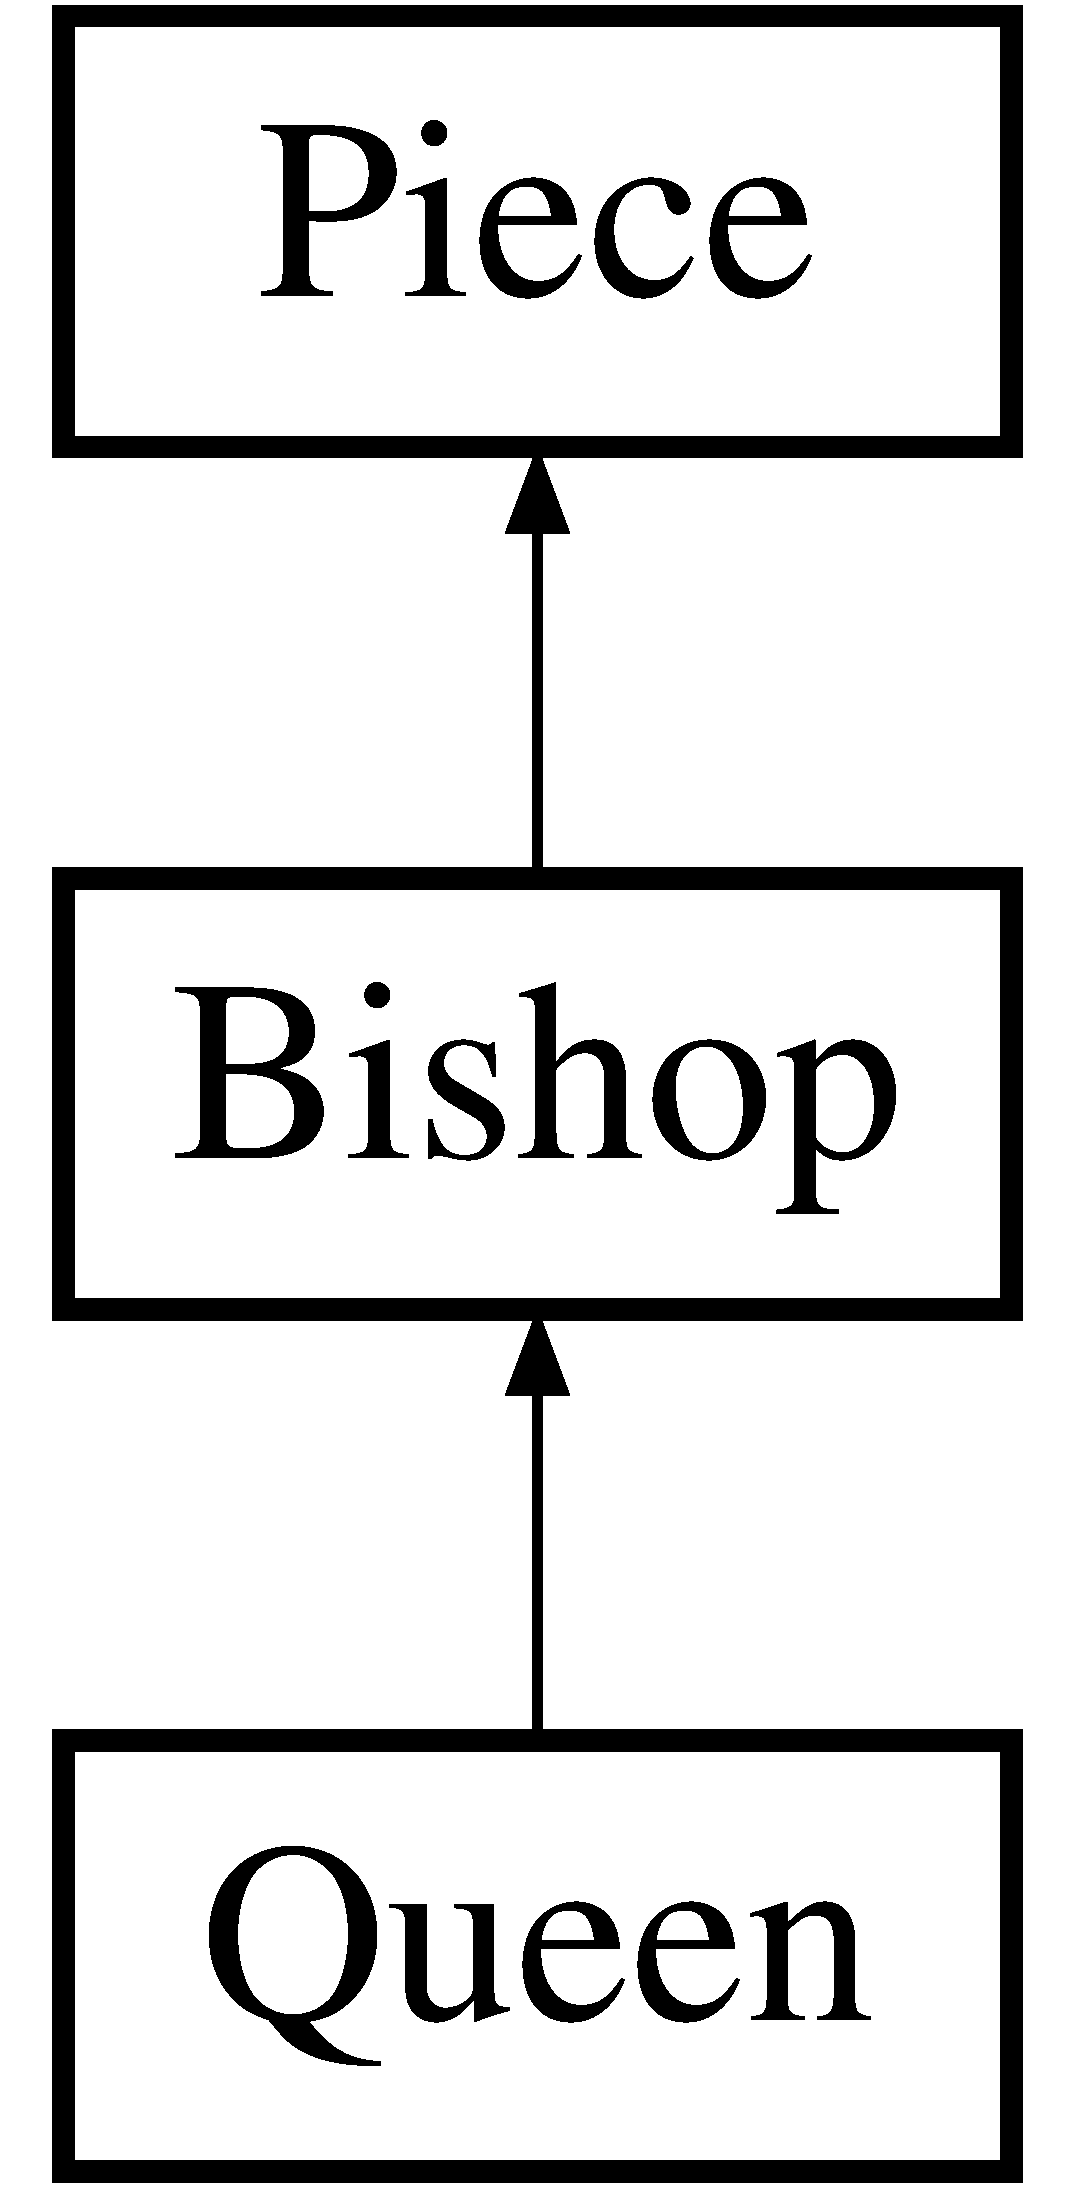
\includegraphics[height=3.000000cm]{class_bishop}
\end{center}
\end{figure}
\subsection*{Public Member Functions}
\begin{DoxyCompactItemize}
\item 
\hyperlink{class_bishop_af4568da25142a681c699ee046e3a630b}{Bishop} ()
\item 
\hyperlink{class_bishop_adf07e0993c6cc5b99aa326cde0e32e95}{Bishop} (string \hyperlink{class_piece_a1b93d0ecc14e15fc7f3fb5def518502a}{position})
\item 
virtual \hyperlink{class_bishop_a3705b4537a39d09a59143fe01a62442f}{$\sim$\+Bishop} ()
\item 
vector$<$ string $>$ \hyperlink{class_bishop_aa5f69fac3ca28996f5c40e34f68822be}{get\+Avail\+Positions} (\hyperlink{class_piece}{Piece} $\ast$$\ast$all)
\end{DoxyCompactItemize}
\subsection*{Additional Inherited Members}


\subsection{Detailed Description}


Definition at line 23 of file Bishop.\+h.



\subsection{Constructor \& Destructor Documentation}
\index{Bishop@{Bishop}!Bishop@{Bishop}}
\index{Bishop@{Bishop}!Bishop@{Bishop}}
\subsubsection[{\texorpdfstring{Bishop()}{Bishop()}}]{\setlength{\rightskip}{0pt plus 5cm}Bishop\+::\+Bishop (
\begin{DoxyParamCaption}
{}
\end{DoxyParamCaption}
)}\hypertarget{class_bishop_af4568da25142a681c699ee046e3a630b}{}\label{class_bishop_af4568da25142a681c699ee046e3a630b}
\index{Bishop@{Bishop}!Bishop@{Bishop}}
\index{Bishop@{Bishop}!Bishop@{Bishop}}
\subsubsection[{\texorpdfstring{Bishop(string position)}{Bishop(string position)}}]{\setlength{\rightskip}{0pt plus 5cm}Bishop\+::\+Bishop (
\begin{DoxyParamCaption}
\item[{string}]{position}
\end{DoxyParamCaption}
)\hspace{0.3cm}{\ttfamily [inline]}}\hypertarget{class_bishop_adf07e0993c6cc5b99aa326cde0e32e95}{}\label{class_bishop_adf07e0993c6cc5b99aa326cde0e32e95}


Definition at line 27 of file Bishop.\+h.

\index{Bishop@{Bishop}!````~Bishop@{$\sim$\+Bishop}}
\index{````~Bishop@{$\sim$\+Bishop}!Bishop@{Bishop}}
\subsubsection[{\texorpdfstring{$\sim$\+Bishop()}{~Bishop()}}]{\setlength{\rightskip}{0pt plus 5cm}Bishop\+::$\sim$\+Bishop (
\begin{DoxyParamCaption}
{}
\end{DoxyParamCaption}
)\hspace{0.3cm}{\ttfamily [virtual]}}\hypertarget{class_bishop_a3705b4537a39d09a59143fe01a62442f}{}\label{class_bishop_a3705b4537a39d09a59143fe01a62442f}


Definition at line 11 of file Bishop.\+cpp.



\subsection{Member Function Documentation}
\index{Bishop@{Bishop}!get\+Avail\+Positions@{get\+Avail\+Positions}}
\index{get\+Avail\+Positions@{get\+Avail\+Positions}!Bishop@{Bishop}}
\subsubsection[{\texorpdfstring{get\+Avail\+Positions(\+Piece $\ast$$\ast$all)}{getAvailPositions(Piece **all)}}]{\setlength{\rightskip}{0pt plus 5cm}vector$<$string$>$ Bishop\+::get\+Avail\+Positions (
\begin{DoxyParamCaption}
\item[{{\bf Piece} $\ast$$\ast$}]{all}
\end{DoxyParamCaption}
)\hspace{0.3cm}{\ttfamily [inline]}, {\ttfamily [virtual]}}\hypertarget{class_bishop_aa5f69fac3ca28996f5c40e34f68822be}{}\label{class_bishop_aa5f69fac3ca28996f5c40e34f68822be}


Implements \hyperlink{class_piece_a4c717dfd8c910e2088bee2c4c6792c10}{Piece}.



Reimplemented in \hyperlink{class_queen_ac9d5264dfe75162fa10e717b3962fdaf}{Queen}.



Definition at line 33 of file Bishop.\+h.



The documentation for this class was generated from the following files\+:\begin{DoxyCompactItemize}
\item 
\hyperlink{_bishop_8h}{Bishop.\+h}\item 
\hyperlink{_bishop_8cpp}{Bishop.\+cpp}\end{DoxyCompactItemize}

\hypertarget{class_king}{}\section{King Class Reference}
\label{class_king}\index{King@{King}}


{\ttfamily \#include $<$King.\+h$>$}

Inheritance diagram for King\+:\begin{figure}[H]
\begin{center}
\leavevmode
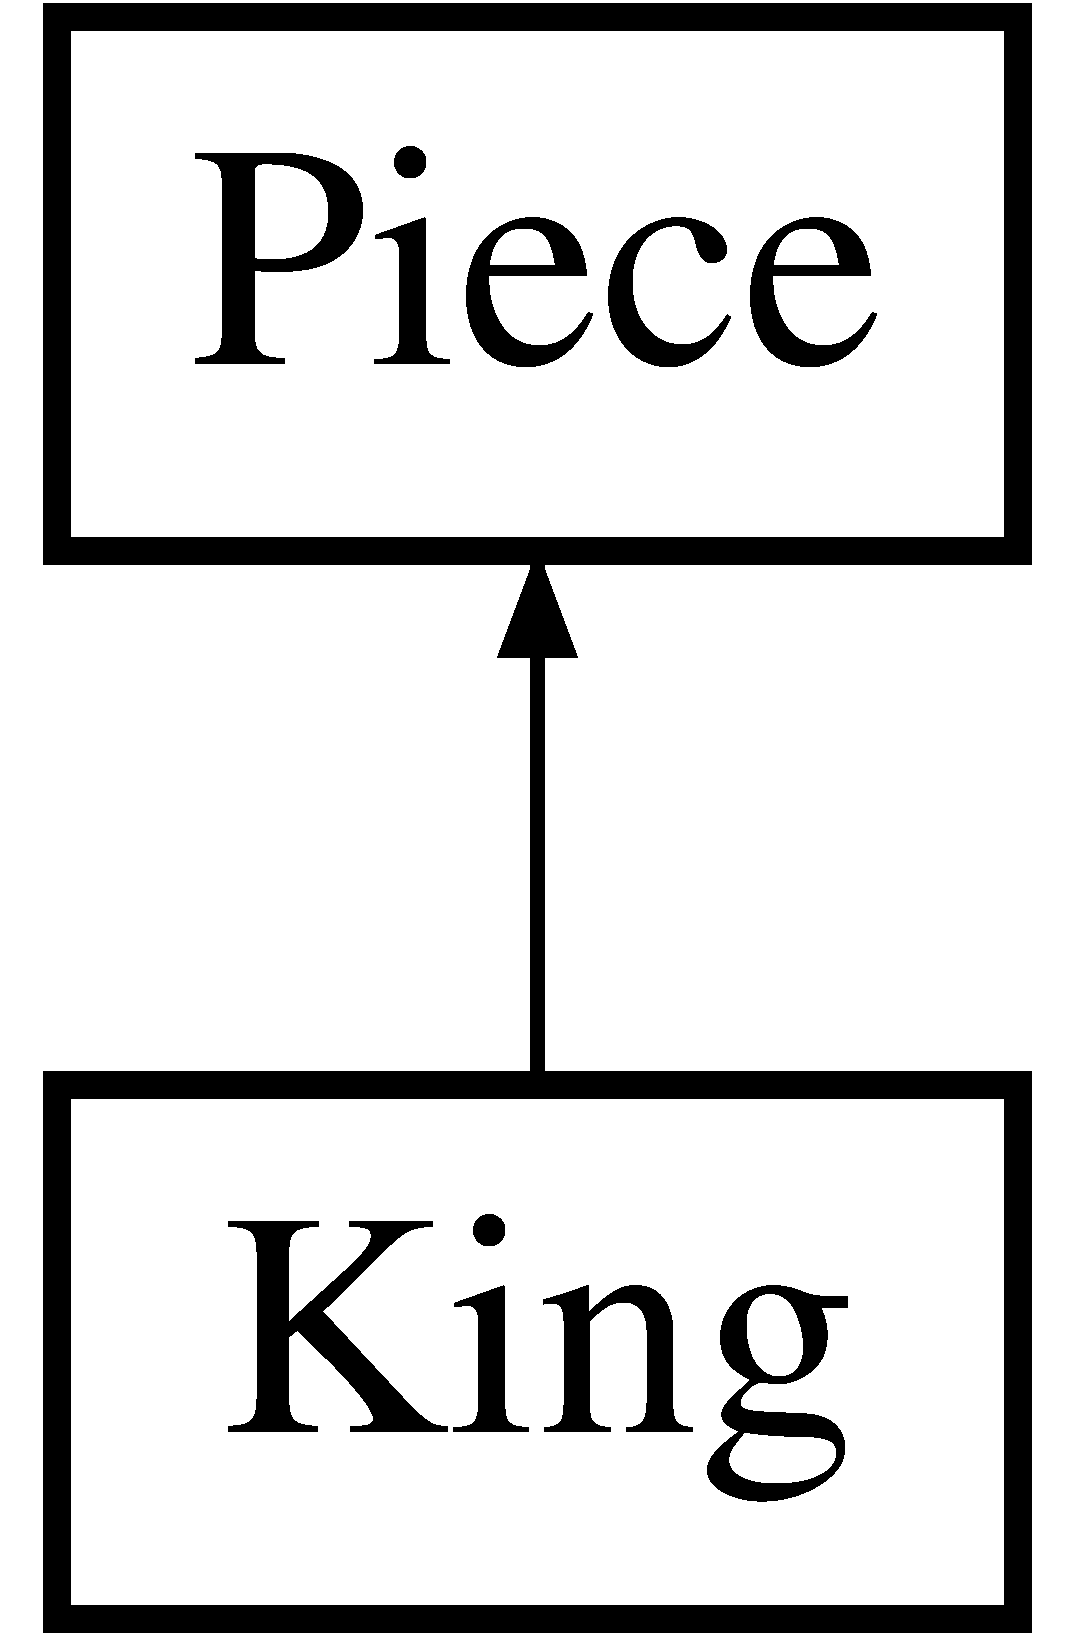
\includegraphics[height=2.000000cm]{class_king}
\end{center}
\end{figure}
\subsection*{Public Member Functions}
\begin{DoxyCompactItemize}
\item 
\hyperlink{class_king_ae374efc047c95212f78a49c877e34563}{King} ()
\item 
\hyperlink{class_king_a3bc5b94579c5895795a55f1ce7a796f4}{King} (string \hyperlink{class_piece_a1b93d0ecc14e15fc7f3fb5def518502a}{position})
\item 
virtual \hyperlink{class_king_aac368ce96e2b12f62e3608d27262e941}{$\sim$\+King} ()
\item 
vector$<$ string $>$ \hyperlink{class_king_aa4d67d5f446902213730ff76a6faab54}{get\+Avail\+Positions} (\hyperlink{class_piece}{Piece} $\ast$$\ast$all)
\end{DoxyCompactItemize}
\subsection*{Additional Inherited Members}


\subsection{Detailed Description}


Definition at line 18 of file King.\+h.



\subsection{Constructor \& Destructor Documentation}
\index{King@{King}!King@{King}}
\index{King@{King}!King@{King}}
\subsubsection[{\texorpdfstring{King()}{King()}}]{\setlength{\rightskip}{0pt plus 5cm}King\+::\+King (
\begin{DoxyParamCaption}
{}
\end{DoxyParamCaption}
)}\hypertarget{class_king_ae374efc047c95212f78a49c877e34563}{}\label{class_king_ae374efc047c95212f78a49c877e34563}
\index{King@{King}!King@{King}}
\index{King@{King}!King@{King}}
\subsubsection[{\texorpdfstring{King(string position)}{King(string position)}}]{\setlength{\rightskip}{0pt plus 5cm}King\+::\+King (
\begin{DoxyParamCaption}
\item[{string}]{position}
\end{DoxyParamCaption}
)\hspace{0.3cm}{\ttfamily [inline]}}\hypertarget{class_king_a3bc5b94579c5895795a55f1ce7a796f4}{}\label{class_king_a3bc5b94579c5895795a55f1ce7a796f4}


Definition at line 22 of file King.\+h.

\index{King@{King}!````~King@{$\sim$\+King}}
\index{````~King@{$\sim$\+King}!King@{King}}
\subsubsection[{\texorpdfstring{$\sim$\+King()}{~King()}}]{\setlength{\rightskip}{0pt plus 5cm}King\+::$\sim$\+King (
\begin{DoxyParamCaption}
{}
\end{DoxyParamCaption}
)\hspace{0.3cm}{\ttfamily [virtual]}}\hypertarget{class_king_aac368ce96e2b12f62e3608d27262e941}{}\label{class_king_aac368ce96e2b12f62e3608d27262e941}


Definition at line 11 of file King.\+cpp.



\subsection{Member Function Documentation}
\index{King@{King}!get\+Avail\+Positions@{get\+Avail\+Positions}}
\index{get\+Avail\+Positions@{get\+Avail\+Positions}!King@{King}}
\subsubsection[{\texorpdfstring{get\+Avail\+Positions(\+Piece $\ast$$\ast$all)}{getAvailPositions(Piece **all)}}]{\setlength{\rightskip}{0pt plus 5cm}vector$<$string$>$ King\+::get\+Avail\+Positions (
\begin{DoxyParamCaption}
\item[{{\bf Piece} $\ast$$\ast$}]{all}
\end{DoxyParamCaption}
)\hspace{0.3cm}{\ttfamily [inline]}, {\ttfamily [virtual]}}\hypertarget{class_king_aa4d67d5f446902213730ff76a6faab54}{}\label{class_king_aa4d67d5f446902213730ff76a6faab54}


Implements \hyperlink{class_piece_a4c717dfd8c910e2088bee2c4c6792c10}{Piece}.



Definition at line 28 of file King.\+h.



The documentation for this class was generated from the following files\+:\begin{DoxyCompactItemize}
\item 
\hyperlink{_king_8h}{King.\+h}\item 
\hyperlink{_king_8cpp}{King.\+cpp}\end{DoxyCompactItemize}

\hypertarget{class_knight}{}\section{Knight Class Reference}
\label{class_knight}\index{Knight@{Knight}}


{\ttfamily \#include $<$Knight.\+h$>$}

Inheritance diagram for Knight\+:\begin{figure}[H]
\begin{center}
\leavevmode
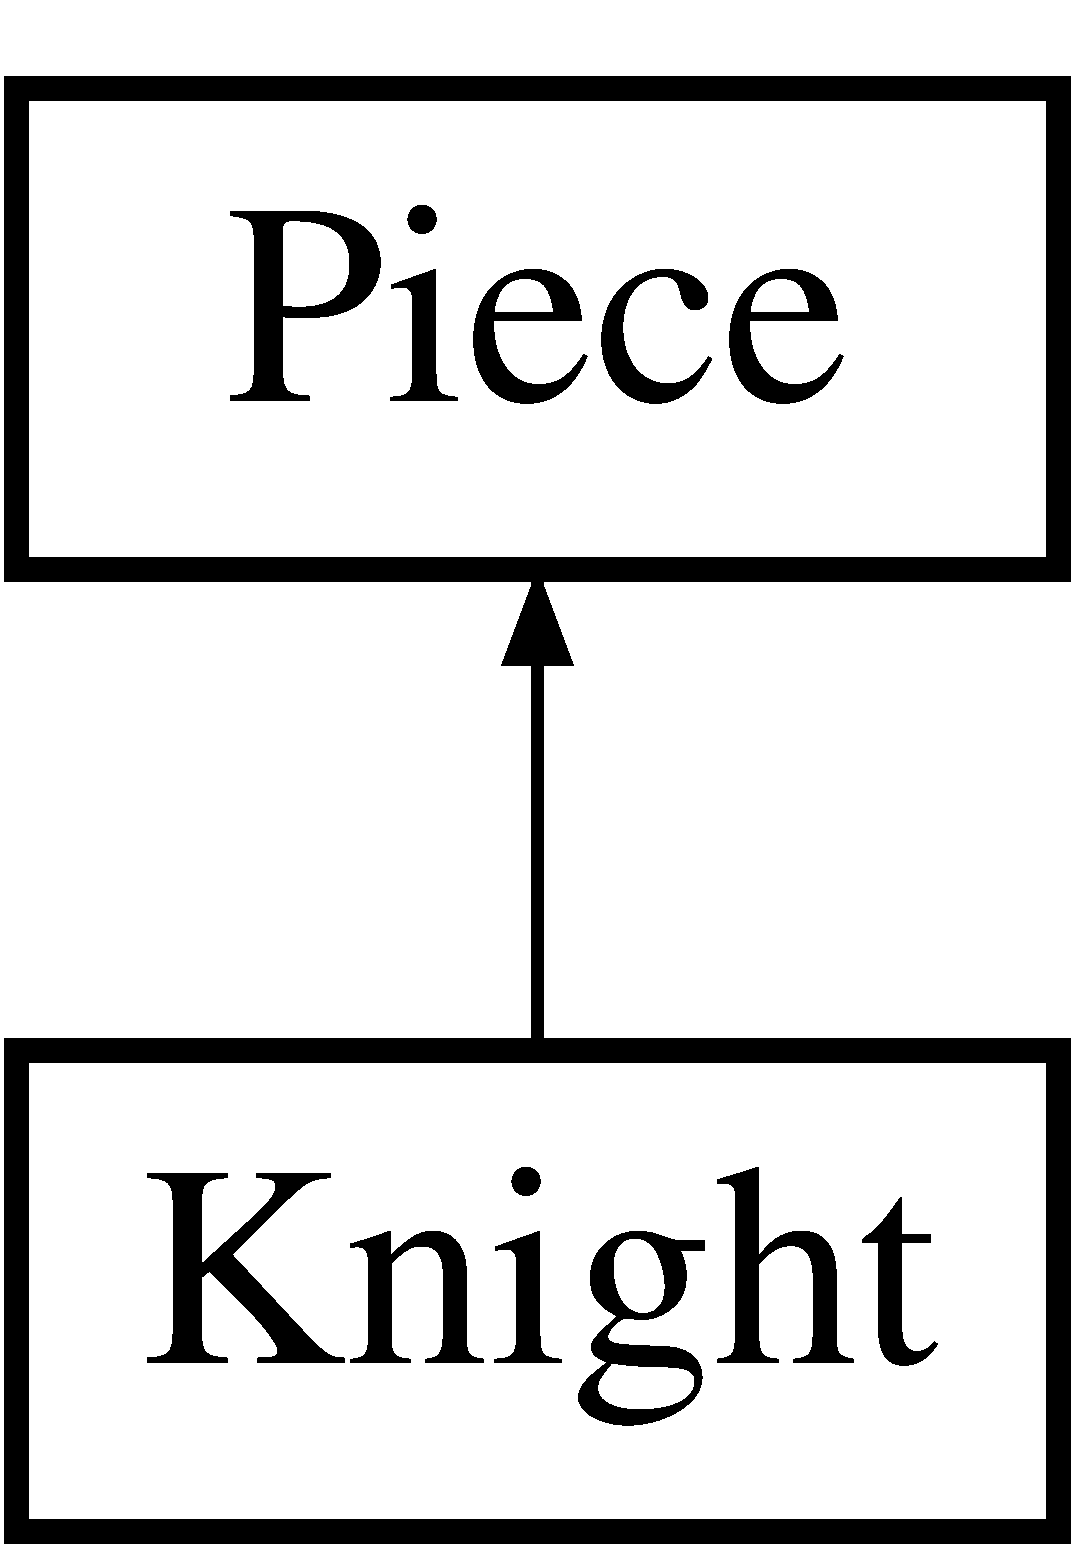
\includegraphics[height=2.000000cm]{class_knight}
\end{center}
\end{figure}
\subsection*{Public Member Functions}
\begin{DoxyCompactItemize}
\item 
\hyperlink{class_knight_aa5c98808cbb05f2772bc3a32ef859387}{Knight} ()
\item 
\hyperlink{class_knight_ae6d6c2e4445aea841a368e2346479481}{Knight} (string \hyperlink{class_piece_a1b93d0ecc14e15fc7f3fb5def518502a}{position})
\item 
virtual \hyperlink{class_knight_a2754123d6876babe915f4da8f761361b}{$\sim$\+Knight} ()
\item 
vector$<$ string $>$ \hyperlink{class_knight_abef9508ede89c70a482ecdd3f08a9d04}{get\+Avail\+Positions} (\hyperlink{class_piece}{Piece} $\ast$$\ast$all) override
\end{DoxyCompactItemize}
\subsection*{Additional Inherited Members}


\subsection{Detailed Description}


Definition at line 18 of file Knight.\+h.



\subsection{Constructor \& Destructor Documentation}
\index{Knight@{Knight}!Knight@{Knight}}
\index{Knight@{Knight}!Knight@{Knight}}
\subsubsection[{\texorpdfstring{Knight()}{Knight()}}]{\setlength{\rightskip}{0pt plus 5cm}Knight\+::\+Knight (
\begin{DoxyParamCaption}
{}
\end{DoxyParamCaption}
)}\hypertarget{class_knight_aa5c98808cbb05f2772bc3a32ef859387}{}\label{class_knight_aa5c98808cbb05f2772bc3a32ef859387}
\index{Knight@{Knight}!Knight@{Knight}}
\index{Knight@{Knight}!Knight@{Knight}}
\subsubsection[{\texorpdfstring{Knight(string position)}{Knight(string position)}}]{\setlength{\rightskip}{0pt plus 5cm}Knight\+::\+Knight (
\begin{DoxyParamCaption}
\item[{string}]{position}
\end{DoxyParamCaption}
)\hspace{0.3cm}{\ttfamily [inline]}}\hypertarget{class_knight_ae6d6c2e4445aea841a368e2346479481}{}\label{class_knight_ae6d6c2e4445aea841a368e2346479481}


Definition at line 22 of file Knight.\+h.

\index{Knight@{Knight}!````~Knight@{$\sim$\+Knight}}
\index{````~Knight@{$\sim$\+Knight}!Knight@{Knight}}
\subsubsection[{\texorpdfstring{$\sim$\+Knight()}{~Knight()}}]{\setlength{\rightskip}{0pt plus 5cm}Knight\+::$\sim$\+Knight (
\begin{DoxyParamCaption}
{}
\end{DoxyParamCaption}
)\hspace{0.3cm}{\ttfamily [virtual]}}\hypertarget{class_knight_a2754123d6876babe915f4da8f761361b}{}\label{class_knight_a2754123d6876babe915f4da8f761361b}


Definition at line 12 of file Knight.\+cpp.



\subsection{Member Function Documentation}
\index{Knight@{Knight}!get\+Avail\+Positions@{get\+Avail\+Positions}}
\index{get\+Avail\+Positions@{get\+Avail\+Positions}!Knight@{Knight}}
\subsubsection[{\texorpdfstring{get\+Avail\+Positions(\+Piece $\ast$$\ast$all) override}{getAvailPositions(Piece **all) override}}]{\setlength{\rightskip}{0pt plus 5cm}vector$<$string$>$ Knight\+::get\+Avail\+Positions (
\begin{DoxyParamCaption}
\item[{{\bf Piece} $\ast$$\ast$}]{all}
\end{DoxyParamCaption}
)\hspace{0.3cm}{\ttfamily [inline]}, {\ttfamily [override]}, {\ttfamily [virtual]}}\hypertarget{class_knight_abef9508ede89c70a482ecdd3f08a9d04}{}\label{class_knight_abef9508ede89c70a482ecdd3f08a9d04}


Implements \hyperlink{class_piece_a4c717dfd8c910e2088bee2c4c6792c10}{Piece}.



Definition at line 28 of file Knight.\+h.



The documentation for this class was generated from the following files\+:\begin{DoxyCompactItemize}
\item 
\hyperlink{_knight_8h}{Knight.\+h}\item 
\hyperlink{_knight_8cpp}{Knight.\+cpp}\end{DoxyCompactItemize}

\hypertarget{class_pawn}{}\section{Pawn Class Reference}
\label{class_pawn}\index{Pawn@{Pawn}}


{\ttfamily \#include $<$Pawn.\+h$>$}

Inheritance diagram for Pawn\+:\begin{figure}[H]
\begin{center}
\leavevmode
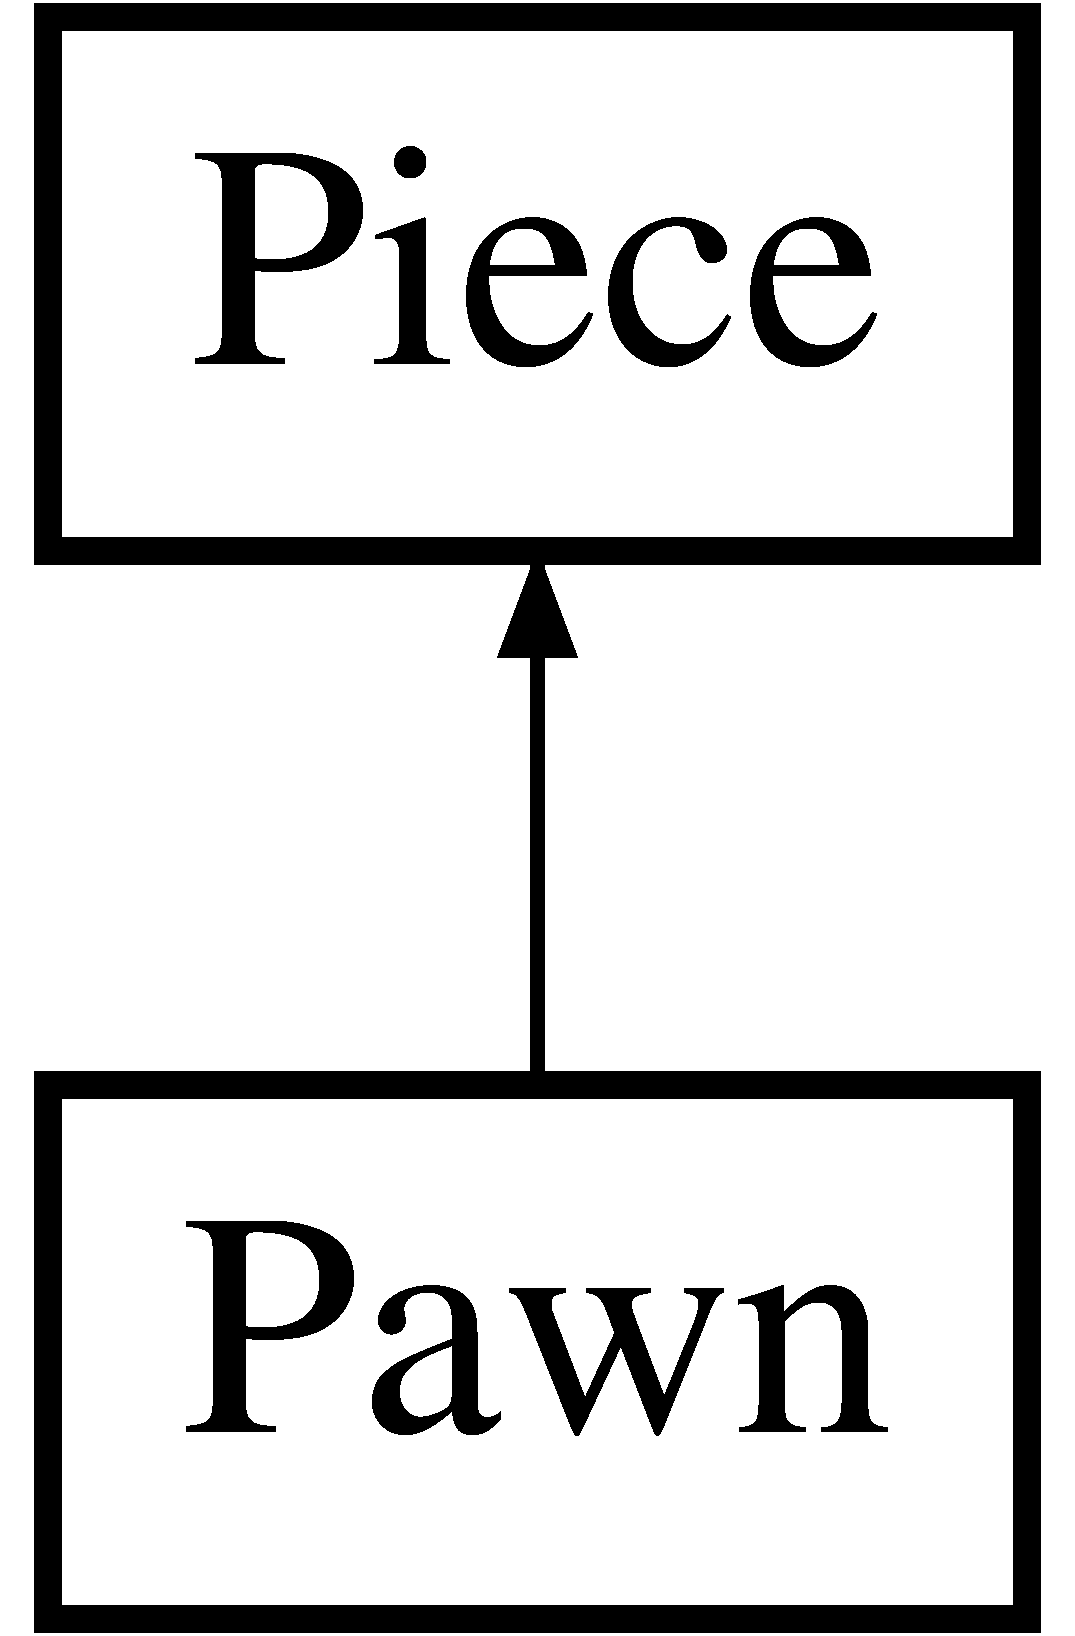
\includegraphics[height=2.000000cm]{class_pawn}
\end{center}
\end{figure}
\subsection*{Public Member Functions}
\begin{DoxyCompactItemize}
\item 
\hyperlink{class_pawn_ab7880b10c514f4b9fab9766fbe7c06fd}{Pawn} ()
\item 
\hyperlink{class_pawn_ad99c9b105e0b0d5fbb479959730422e2}{Pawn} (string \hyperlink{class_piece_a1b93d0ecc14e15fc7f3fb5def518502a}{position})
\item 
virtual \hyperlink{class_pawn_a3095938fb8326469c3bd05da0b8f50af}{$\sim$\+Pawn} ()
\item 
vector$<$ string $>$ \hyperlink{class_pawn_a140eb39f4412a235d3e1ab5f533725e8}{get\+Avail\+Positions} (\hyperlink{class_piece}{Piece} $\ast$$\ast$all) override
\end{DoxyCompactItemize}
\subsection*{Additional Inherited Members}


\subsection{Detailed Description}


Definition at line 18 of file Pawn.\+h.



\subsection{Constructor \& Destructor Documentation}
\index{Pawn@{Pawn}!Pawn@{Pawn}}
\index{Pawn@{Pawn}!Pawn@{Pawn}}
\subsubsection[{\texorpdfstring{Pawn()}{Pawn()}}]{\setlength{\rightskip}{0pt plus 5cm}Pawn\+::\+Pawn (
\begin{DoxyParamCaption}
{}
\end{DoxyParamCaption}
)}\hypertarget{class_pawn_ab7880b10c514f4b9fab9766fbe7c06fd}{}\label{class_pawn_ab7880b10c514f4b9fab9766fbe7c06fd}
\index{Pawn@{Pawn}!Pawn@{Pawn}}
\index{Pawn@{Pawn}!Pawn@{Pawn}}
\subsubsection[{\texorpdfstring{Pawn(string position)}{Pawn(string position)}}]{\setlength{\rightskip}{0pt plus 5cm}Pawn\+::\+Pawn (
\begin{DoxyParamCaption}
\item[{string}]{position}
\end{DoxyParamCaption}
)\hspace{0.3cm}{\ttfamily [inline]}}\hypertarget{class_pawn_ad99c9b105e0b0d5fbb479959730422e2}{}\label{class_pawn_ad99c9b105e0b0d5fbb479959730422e2}


Definition at line 22 of file Pawn.\+h.

\index{Pawn@{Pawn}!````~Pawn@{$\sim$\+Pawn}}
\index{````~Pawn@{$\sim$\+Pawn}!Pawn@{Pawn}}
\subsubsection[{\texorpdfstring{$\sim$\+Pawn()}{~Pawn()}}]{\setlength{\rightskip}{0pt plus 5cm}Pawn\+::$\sim$\+Pawn (
\begin{DoxyParamCaption}
{}
\end{DoxyParamCaption}
)\hspace{0.3cm}{\ttfamily [virtual]}}\hypertarget{class_pawn_a3095938fb8326469c3bd05da0b8f50af}{}\label{class_pawn_a3095938fb8326469c3bd05da0b8f50af}


Definition at line 11 of file Pawn.\+cpp.



\subsection{Member Function Documentation}
\index{Pawn@{Pawn}!get\+Avail\+Positions@{get\+Avail\+Positions}}
\index{get\+Avail\+Positions@{get\+Avail\+Positions}!Pawn@{Pawn}}
\subsubsection[{\texorpdfstring{get\+Avail\+Positions(\+Piece $\ast$$\ast$all) override}{getAvailPositions(Piece **all) override}}]{\setlength{\rightskip}{0pt plus 5cm}vector$<$string$>$ Pawn\+::get\+Avail\+Positions (
\begin{DoxyParamCaption}
\item[{{\bf Piece} $\ast$$\ast$}]{all}
\end{DoxyParamCaption}
)\hspace{0.3cm}{\ttfamily [inline]}, {\ttfamily [override]}, {\ttfamily [virtual]}}\hypertarget{class_pawn_a140eb39f4412a235d3e1ab5f533725e8}{}\label{class_pawn_a140eb39f4412a235d3e1ab5f533725e8}


Implements \hyperlink{class_piece_a4c717dfd8c910e2088bee2c4c6792c10}{Piece}.



Definition at line 27 of file Pawn.\+h.



The documentation for this class was generated from the following files\+:\begin{DoxyCompactItemize}
\item 
\hyperlink{_pawn_8h}{Pawn.\+h}\item 
\hyperlink{_pawn_8cpp}{Pawn.\+cpp}\end{DoxyCompactItemize}

\hypertarget{class_piece}{}\section{Piece Class Reference}
\label{class_piece}\index{Piece@{Piece}}


{\ttfamily \#include $<$Piece.\+h$>$}

Inheritance diagram for Piece\+:\begin{figure}[H]
\begin{center}
\leavevmode
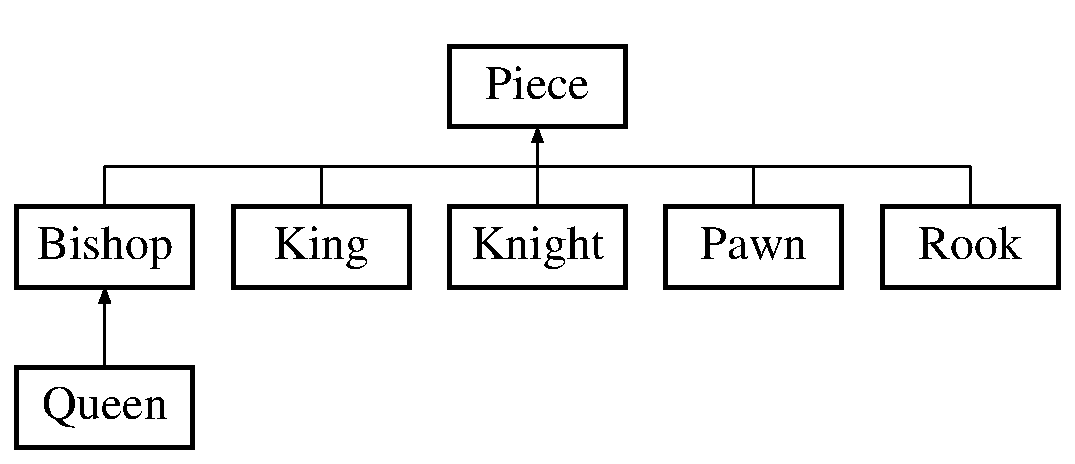
\includegraphics[height=3.000000cm]{class_piece}
\end{center}
\end{figure}
\subsection*{Public Member Functions}
\begin{DoxyCompactItemize}
\item 
\hyperlink{class_piece_a8b0e865b1cfdc0e87ececdd80febfe9a}{Piece} (string \hyperlink{class_piece_a1b93d0ecc14e15fc7f3fb5def518502a}{position})
\item 
virtual \hyperlink{class_piece_a5d7a4f6bade94cb33b6f634de8aa7918}{$\sim$\+Piece} ()
\item 
string \hyperlink{class_piece_a4fa31a8bbea35a6ce0fde5d52d96774b}{get\+Position} ()
\item 
void \hyperlink{class_piece_a64c41f989409d75c48949519aa3e7d38}{set\+Position} (string \hyperlink{class_piece_a1b93d0ecc14e15fc7f3fb5def518502a}{position})
\item 
string \hyperlink{class_piece_a298e07af4a4cb4b8d180e92afd70ffe9}{get\+Symbol} ()
\item 
void \hyperlink{class_piece_ac82f95ec7d998195bdd011a8ee2f3204}{set\+Symbol} (char \hyperlink{class_piece_ab1063e521716374d9a97eddf169be096}{symbol})
\item 
void \hyperlink{class_piece_af60f38fc97d33416b6286d5e74c33778}{move} (\hyperlink{class_piece}{Piece} $\ast$$\ast$all, fstream \&f, map$<$ string, int $>$ \&m, string input, string input2)
\item 
\hyperlink{class_piece}{Piece} $\ast$ \hyperlink{class_piece_acd99f07eb824e56af8e2025d68efafd3}{get\+Piece\+For\+Pos} (\hyperlink{class_piece}{Piece} $\ast$$\ast$all, string s)
\item 
virtual vector$<$ string $>$ \hyperlink{class_piece_a4c717dfd8c910e2088bee2c4c6792c10}{get\+Avail\+Positions} (\hyperlink{class_piece}{Piece} $\ast$$\ast$all)=0
\end{DoxyCompactItemize}
\subsection*{Static Public Member Functions}
\begin{DoxyCompactItemize}
\item 
static void \hyperlink{class_piece_a0cd78824f4ad57ce5772ddaf28b152b0}{draw\+Pieces} (fstream \&file, map$<$ string, int $>$ \&m, \hyperlink{class_piece}{Piece} $\ast$$\ast$pieces, short iters)
\end{DoxyCompactItemize}
\subsection*{Protected Member Functions}
\begin{DoxyCompactItemize}
\item 
void \hyperlink{class_piece_a4e89ae7011b06d46dc4ba76b6f676791}{remove\+Invalids} (vector$<$ string $>$ \&v)
\item 
void \hyperlink{class_piece_a5af40f3573b8963bdd202a750268c3e9}{rmv\+Same\+Symb} (\hyperlink{class_piece}{Piece} $\ast$$\ast$piece, vector$<$ string $>$ \&v)
\item 
bool \hyperlink{class_piece_afbd16578f663257d4dea5beefcdcecb4}{is\+Occ} (\hyperlink{class_piece}{Piece} $\ast$$\ast$all, string s)
\item 
bool \hyperlink{class_piece_afc9b134f63e2b3d5891e2ba0699edf95}{same\+Symb} (string s)
\end{DoxyCompactItemize}
\subsection*{Protected Attributes}
\begin{DoxyCompactItemize}
\item 
string \hyperlink{class_piece_ab1063e521716374d9a97eddf169be096}{symbol}
\item 
string \hyperlink{class_piece_a1b93d0ecc14e15fc7f3fb5def518502a}{position}
\item 
vector$<$ string $>$ \hyperlink{class_piece_aba40a894958b12d2e9f2d3b8ac192316}{avail\+Positions}
\end{DoxyCompactItemize}
\subsection*{Static Protected Attributes}
\begin{DoxyCompactItemize}
\item 
static char \hyperlink{class_piece_af96dfaa19d200cac55748774dbb1a56a}{valids} \mbox{[}16\mbox{]}
\end{DoxyCompactItemize}


\subsection{Detailed Description}


Definition at line 22 of file Piece.\+h.



\subsection{Constructor \& Destructor Documentation}
\index{Piece@{Piece}!Piece@{Piece}}
\index{Piece@{Piece}!Piece@{Piece}}
\subsubsection[{\texorpdfstring{Piece(string position)}{Piece(string position)}}]{\setlength{\rightskip}{0pt plus 5cm}Piece\+::\+Piece (
\begin{DoxyParamCaption}
\item[{string}]{position}
\end{DoxyParamCaption}
)}\hypertarget{class_piece_a8b0e865b1cfdc0e87ececdd80febfe9a}{}\label{class_piece_a8b0e865b1cfdc0e87ececdd80febfe9a}
Construct a \hyperlink{class_piece}{Piece} at a given position coordinate. 
\begin{DoxyParams}{Parameters}
{\em position} & \\
\hline
\end{DoxyParams}


Definition at line 15 of file Piece.\+cpp.

\index{Piece@{Piece}!````~Piece@{$\sim$\+Piece}}
\index{````~Piece@{$\sim$\+Piece}!Piece@{Piece}}
\subsubsection[{\texorpdfstring{$\sim$\+Piece()}{~Piece()}}]{\setlength{\rightskip}{0pt plus 5cm}Piece\+::$\sim$\+Piece (
\begin{DoxyParamCaption}
{}
\end{DoxyParamCaption}
)\hspace{0.3cm}{\ttfamily [virtual]}}\hypertarget{class_piece_a5d7a4f6bade94cb33b6f634de8aa7918}{}\label{class_piece_a5d7a4f6bade94cb33b6f634de8aa7918}


Definition at line 20 of file Piece.\+cpp.



\subsection{Member Function Documentation}
\index{Piece@{Piece}!draw\+Pieces@{draw\+Pieces}}
\index{draw\+Pieces@{draw\+Pieces}!Piece@{Piece}}
\subsubsection[{\texorpdfstring{draw\+Pieces(fstream \&file, map$<$ string, int $>$ \&m, Piece $\ast$$\ast$pieces, short iters)}{drawPieces(fstream &file, map< string, int > &m, Piece **pieces, short iters)}}]{\setlength{\rightskip}{0pt plus 5cm}void Piece\+::draw\+Pieces (
\begin{DoxyParamCaption}
\item[{fstream \&}]{file, }
\item[{map$<$ string, int $>$ \&}]{m, }
\item[{{\bf Piece} $\ast$$\ast$}]{pieces, }
\item[{short}]{iters}
\end{DoxyParamCaption}
)\hspace{0.3cm}{\ttfamily [static]}}\hypertarget{class_piece_a0cd78824f4ad57ce5772ddaf28b152b0}{}\label{class_piece_a0cd78824f4ad57ce5772ddaf28b152b0}
Write a number of Pieces to the game file. Ignore if \hyperlink{class_piece}{Piece} was captured. 
\begin{DoxyParams}{Parameters}
{\em file} & The game file. \\
\hline
{\em m} & The coordinates map. \\
\hline
{\em pieces} & The Pieces to draw. \\
\hline
{\em iters} & The number of Pieces. \\
\hline
\end{DoxyParams}


Definition at line 80 of file Piece.\+cpp.

\index{Piece@{Piece}!get\+Avail\+Positions@{get\+Avail\+Positions}}
\index{get\+Avail\+Positions@{get\+Avail\+Positions}!Piece@{Piece}}
\subsubsection[{\texorpdfstring{get\+Avail\+Positions(\+Piece $\ast$$\ast$all)=0}{getAvailPositions(Piece **all)=0}}]{\setlength{\rightskip}{0pt plus 5cm}virtual vector$<$string$>$ Piece\+::get\+Avail\+Positions (
\begin{DoxyParamCaption}
\item[{{\bf Piece} $\ast$$\ast$}]{all}
\end{DoxyParamCaption}
)\hspace{0.3cm}{\ttfamily [pure virtual]}}\hypertarget{class_piece_a4c717dfd8c910e2088bee2c4c6792c10}{}\label{class_piece_a4c717dfd8c910e2088bee2c4c6792c10}


Implemented in \hyperlink{class_bishop_aa5f69fac3ca28996f5c40e34f68822be}{Bishop}, \hyperlink{class_queen_ac9d5264dfe75162fa10e717b3962fdaf}{Queen}, \hyperlink{class_king_aa4d67d5f446902213730ff76a6faab54}{King}, \hyperlink{class_knight_abef9508ede89c70a482ecdd3f08a9d04}{Knight}, \hyperlink{class_rook_a96e1e49295f230cda98007a7df6d65fa}{Rook}, and \hyperlink{class_pawn_a140eb39f4412a235d3e1ab5f533725e8}{Pawn}.

\index{Piece@{Piece}!get\+Piece\+For\+Pos@{get\+Piece\+For\+Pos}}
\index{get\+Piece\+For\+Pos@{get\+Piece\+For\+Pos}!Piece@{Piece}}
\subsubsection[{\texorpdfstring{get\+Piece\+For\+Pos(\+Piece $\ast$$\ast$all, string s)}{getPieceForPos(Piece **all, string s)}}]{\setlength{\rightskip}{0pt plus 5cm}{\bf Piece} $\ast$ Piece\+::get\+Piece\+For\+Pos (
\begin{DoxyParamCaption}
\item[{{\bf Piece} $\ast$$\ast$}]{all, }
\item[{string}]{s}
\end{DoxyParamCaption}
)}\hypertarget{class_piece_acd99f07eb824e56af8e2025d68efafd3}{}\label{class_piece_acd99f07eb824e56af8e2025d68efafd3}
Gets a \hyperlink{class_piece}{Piece} given a position. 
\begin{DoxyParams}{Parameters}
{\em all} & The 32 Pieces. \\
\hline
{\em s} & The position string. \\
\hline
\end{DoxyParams}
\begin{DoxyReturn}{Returns}
The \hyperlink{class_piece}{Piece} at the specified position, or N\+U\+LL. 
\end{DoxyReturn}


Definition at line 169 of file Piece.\+cpp.

\index{Piece@{Piece}!get\+Position@{get\+Position}}
\index{get\+Position@{get\+Position}!Piece@{Piece}}
\subsubsection[{\texorpdfstring{get\+Position()}{getPosition()}}]{\setlength{\rightskip}{0pt plus 5cm}string Piece\+::get\+Position (
\begin{DoxyParamCaption}
{}
\end{DoxyParamCaption}
)}\hypertarget{class_piece_a4fa31a8bbea35a6ce0fde5d52d96774b}{}\label{class_piece_a4fa31a8bbea35a6ce0fde5d52d96774b}


Definition at line 34 of file Piece.\+cpp.

\index{Piece@{Piece}!get\+Symbol@{get\+Symbol}}
\index{get\+Symbol@{get\+Symbol}!Piece@{Piece}}
\subsubsection[{\texorpdfstring{get\+Symbol()}{getSymbol()}}]{\setlength{\rightskip}{0pt plus 5cm}string Piece\+::get\+Symbol (
\begin{DoxyParamCaption}
{}
\end{DoxyParamCaption}
)}\hypertarget{class_piece_a298e07af4a4cb4b8d180e92afd70ffe9}{}\label{class_piece_a298e07af4a4cb4b8d180e92afd70ffe9}


Definition at line 22 of file Piece.\+cpp.

\index{Piece@{Piece}!is\+Occ@{is\+Occ}}
\index{is\+Occ@{is\+Occ}!Piece@{Piece}}
\subsubsection[{\texorpdfstring{is\+Occ(\+Piece $\ast$$\ast$all, string s)}{isOcc(Piece **all, string s)}}]{\setlength{\rightskip}{0pt plus 5cm}bool Piece\+::is\+Occ (
\begin{DoxyParamCaption}
\item[{{\bf Piece} $\ast$$\ast$}]{all, }
\item[{string}]{s}
\end{DoxyParamCaption}
)\hspace{0.3cm}{\ttfamily [protected]}}\hypertarget{class_piece_afbd16578f663257d4dea5beefcdcecb4}{}\label{class_piece_afbd16578f663257d4dea5beefcdcecb4}
Check if a position is occupied. 
\begin{DoxyParams}{Parameters}
{\em all} & The 32 Pieces. \\
\hline
{\em s} & The position to check. \\
\hline
\end{DoxyParams}
\begin{DoxyReturn}{Returns}
True if position is occupied. False otherwise. 
\end{DoxyReturn}


Definition at line 100 of file Piece.\+cpp.

\index{Piece@{Piece}!move@{move}}
\index{move@{move}!Piece@{Piece}}
\subsubsection[{\texorpdfstring{move(\+Piece $\ast$$\ast$all, fstream \&f, map$<$ string, int $>$ \&m, string input, string input2)}{move(Piece **all, fstream &f, map< string, int > &m, string input, string input2)}}]{\setlength{\rightskip}{0pt plus 5cm}void Piece\+::move (
\begin{DoxyParamCaption}
\item[{{\bf Piece} $\ast$$\ast$}]{all, }
\item[{fstream \&}]{f, }
\item[{map$<$ string, int $>$ \&}]{m, }
\item[{string}]{input, }
\item[{string}]{input2}
\end{DoxyParamCaption}
)}\hypertarget{class_piece_af60f38fc97d33416b6286d5e74c33778}{}\label{class_piece_af60f38fc97d33416b6286d5e74c33778}
Change the position of a \hyperlink{class_piece}{Piece} inside the game file. 
\begin{DoxyParams}{Parameters}
{\em all} & The 32 Pieces. \\
\hline
{\em f} & The file to write to. \\
\hline
{\em m} & The coordinates map. \\
\hline
{\em input} & The selected position. \\
\hline
{\em input2} & The destination position. \\
\hline
\end{DoxyParams}


Definition at line 52 of file Piece.\+cpp.

\index{Piece@{Piece}!remove\+Invalids@{remove\+Invalids}}
\index{remove\+Invalids@{remove\+Invalids}!Piece@{Piece}}
\subsubsection[{\texorpdfstring{remove\+Invalids(vector$<$ string $>$ \&v)}{removeInvalids(vector< string > &v)}}]{\setlength{\rightskip}{0pt plus 5cm}void Piece\+::remove\+Invalids (
\begin{DoxyParamCaption}
\item[{vector$<$ string $>$ \&}]{v}
\end{DoxyParamCaption}
)\hspace{0.3cm}{\ttfamily [protected]}}\hypertarget{class_piece_a4e89ae7011b06d46dc4ba76b6f676791}{}\label{class_piece_a4e89ae7011b06d46dc4ba76b6f676791}
Removes all invalid positions. See \char`\"{}bool invalid(string p)\char`\"{} for details. 
\begin{DoxyParams}{Parameters}
{\em v} & The vector containing valid and invalid positions. \\
\hline
\end{DoxyParams}


Definition at line 134 of file Piece.\+cpp.

\index{Piece@{Piece}!rmv\+Same\+Symb@{rmv\+Same\+Symb}}
\index{rmv\+Same\+Symb@{rmv\+Same\+Symb}!Piece@{Piece}}
\subsubsection[{\texorpdfstring{rmv\+Same\+Symb(\+Piece $\ast$$\ast$piece, vector$<$ string $>$ \&v)}{rmvSameSymb(Piece **piece, vector< string > &v)}}]{\setlength{\rightskip}{0pt plus 5cm}void Piece\+::rmv\+Same\+Symb (
\begin{DoxyParamCaption}
\item[{{\bf Piece} $\ast$$\ast$}]{all, }
\item[{vector$<$ string $>$ \&}]{v}
\end{DoxyParamCaption}
)\hspace{0.3cm}{\ttfamily [protected]}}\hypertarget{class_piece_a5af40f3573b8963bdd202a750268c3e9}{}\label{class_piece_a5af40f3573b8963bdd202a750268c3e9}
Remove positions where our teams pieces are. 
\begin{DoxyParams}{Parameters}
{\em all} & The 32 Pieces. \\
\hline
{\em v} & The vector containing positions of our team and enemies. \\
\hline
\end{DoxyParams}


Definition at line 144 of file Piece.\+cpp.

\index{Piece@{Piece}!same\+Symb@{same\+Symb}}
\index{same\+Symb@{same\+Symb}!Piece@{Piece}}
\subsubsection[{\texorpdfstring{same\+Symb(string s)}{sameSymb(string s)}}]{\setlength{\rightskip}{0pt plus 5cm}bool Piece\+::same\+Symb (
\begin{DoxyParamCaption}
\item[{string}]{s}
\end{DoxyParamCaption}
)\hspace{0.3cm}{\ttfamily [protected]}}\hypertarget{class_piece_afc9b134f63e2b3d5891e2ba0699edf95}{}\label{class_piece_afc9b134f63e2b3d5891e2ba0699edf95}
\index{Piece@{Piece}!set\+Position@{set\+Position}}
\index{set\+Position@{set\+Position}!Piece@{Piece}}
\subsubsection[{\texorpdfstring{set\+Position(string position)}{setPosition(string position)}}]{\setlength{\rightskip}{0pt plus 5cm}void Piece\+::set\+Position (
\begin{DoxyParamCaption}
\item[{string}]{position}
\end{DoxyParamCaption}
)}\hypertarget{class_piece_a64c41f989409d75c48949519aa3e7d38}{}\label{class_piece_a64c41f989409d75c48949519aa3e7d38}


Definition at line 39 of file Piece.\+cpp.

\index{Piece@{Piece}!set\+Symbol@{set\+Symbol}}
\index{set\+Symbol@{set\+Symbol}!Piece@{Piece}}
\subsubsection[{\texorpdfstring{set\+Symbol(char symbol)}{setSymbol(char symbol)}}]{\setlength{\rightskip}{0pt plus 5cm}void Piece\+::set\+Symbol (
\begin{DoxyParamCaption}
\item[{char}]{symbol}
\end{DoxyParamCaption}
)}\hypertarget{class_piece_ac82f95ec7d998195bdd011a8ee2f3204}{}\label{class_piece_ac82f95ec7d998195bdd011a8ee2f3204}


Definition at line 27 of file Piece.\+cpp.



\subsection{Member Data Documentation}
\index{Piece@{Piece}!avail\+Positions@{avail\+Positions}}
\index{avail\+Positions@{avail\+Positions}!Piece@{Piece}}
\subsubsection[{\texorpdfstring{avail\+Positions}{availPositions}}]{\setlength{\rightskip}{0pt plus 5cm}vector$<$string$>$ Piece\+::avail\+Positions\hspace{0.3cm}{\ttfamily [protected]}}\hypertarget{class_piece_aba40a894958b12d2e9f2d3b8ac192316}{}\label{class_piece_aba40a894958b12d2e9f2d3b8ac192316}


Definition at line 40 of file Piece.\+h.

\index{Piece@{Piece}!position@{position}}
\index{position@{position}!Piece@{Piece}}
\subsubsection[{\texorpdfstring{position}{position}}]{\setlength{\rightskip}{0pt plus 5cm}string Piece\+::position\hspace{0.3cm}{\ttfamily [protected]}}\hypertarget{class_piece_a1b93d0ecc14e15fc7f3fb5def518502a}{}\label{class_piece_a1b93d0ecc14e15fc7f3fb5def518502a}


Definition at line 39 of file Piece.\+h.

\index{Piece@{Piece}!symbol@{symbol}}
\index{symbol@{symbol}!Piece@{Piece}}
\subsubsection[{\texorpdfstring{symbol}{symbol}}]{\setlength{\rightskip}{0pt plus 5cm}string Piece\+::symbol\hspace{0.3cm}{\ttfamily [protected]}}\hypertarget{class_piece_ab1063e521716374d9a97eddf169be096}{}\label{class_piece_ab1063e521716374d9a97eddf169be096}


Definition at line 38 of file Piece.\+h.

\index{Piece@{Piece}!valids@{valids}}
\index{valids@{valids}!Piece@{Piece}}
\subsubsection[{\texorpdfstring{valids}{valids}}]{\setlength{\rightskip}{0pt plus 5cm}char Piece\+::valids\hspace{0.3cm}{\ttfamily [static]}, {\ttfamily [protected]}}\hypertarget{class_piece_af96dfaa19d200cac55748774dbb1a56a}{}\label{class_piece_af96dfaa19d200cac55748774dbb1a56a}
{\bfseries Initial value\+:}
\begin{DoxyCode}
= \{
    \textcolor{charliteral}{'A'}, \textcolor{charliteral}{'B'}, \textcolor{charliteral}{'C'}, \textcolor{charliteral}{'D'}, \textcolor{charliteral}{'E'}, \textcolor{charliteral}{'F'}, \textcolor{charliteral}{'G'}, \textcolor{charliteral}{'H'},
    \textcolor{charliteral}{'0'}, \textcolor{charliteral}{'1'}, \textcolor{charliteral}{'2'}, \textcolor{charliteral}{'3'}, \textcolor{charliteral}{'4'}, \textcolor{charliteral}{'5'}, \textcolor{charliteral}{'6'}, \textcolor{charliteral}{'7'}
\}
\end{DoxyCode}
Depreciated. 

Definition at line 41 of file Piece.\+h.



The documentation for this class was generated from the following files\+:\begin{DoxyCompactItemize}
\item 
\hyperlink{_piece_8h}{Piece.\+h}\item 
\hyperlink{_piece_8cpp}{Piece.\+cpp}\end{DoxyCompactItemize}

\hypertarget{class_queen}{}\section{Queen Class Reference}
\label{class_queen}\index{Queen@{Queen}}


{\ttfamily \#include $<$Queen.\+h$>$}

Inheritance diagram for Queen\+:\begin{figure}[H]
\begin{center}
\leavevmode
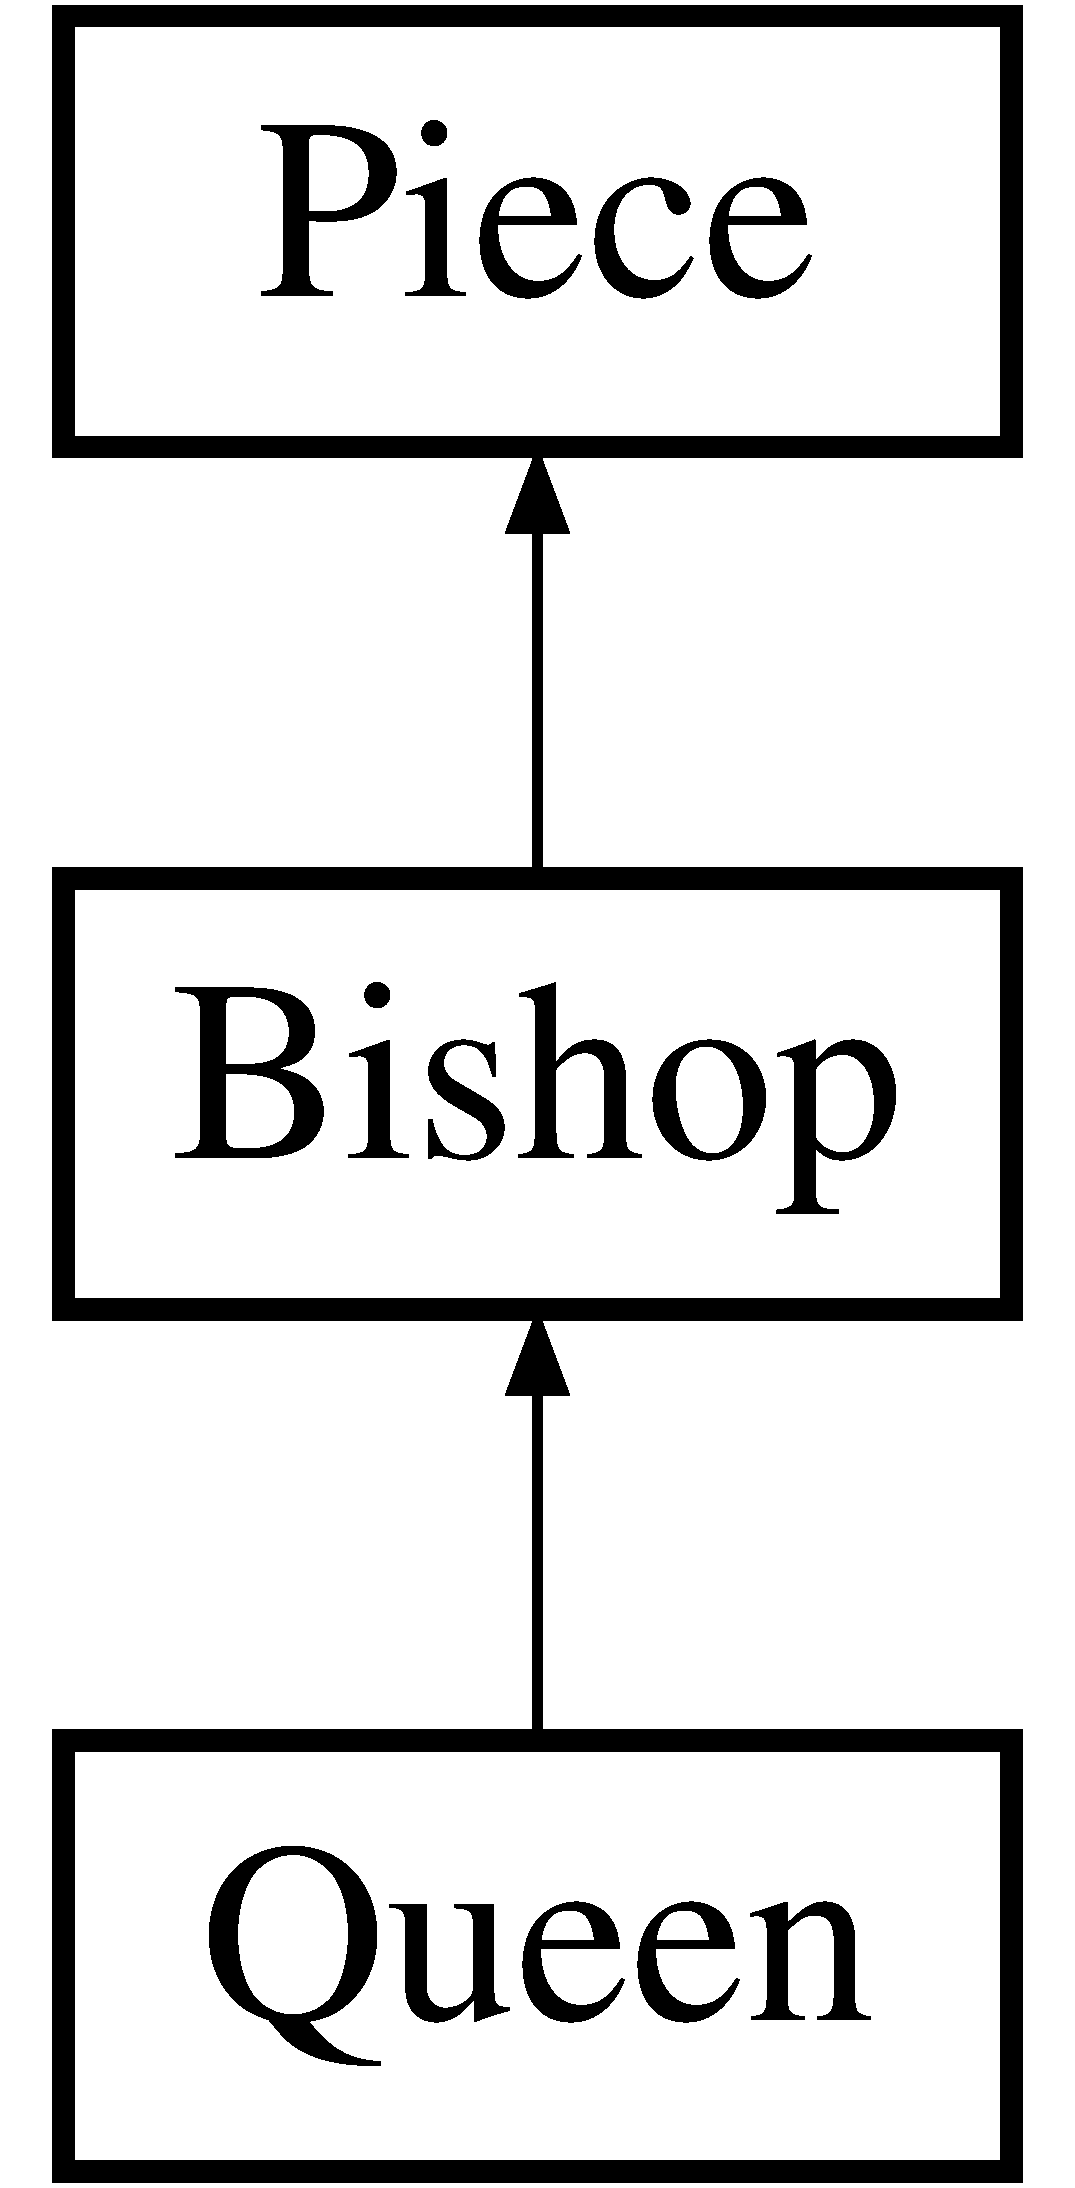
\includegraphics[height=3.000000cm]{class_queen}
\end{center}
\end{figure}
\subsection*{Public Member Functions}
\begin{DoxyCompactItemize}
\item 
\hyperlink{class_queen_ae2314f4890c7fa7d5da670b3c0b6293b}{Queen} ()
\item 
\hyperlink{class_queen_aeff77ee1186113902e6cf60ff6a6cd76}{Queen} (string \hyperlink{class_piece_a1b93d0ecc14e15fc7f3fb5def518502a}{position})
\item 
virtual \hyperlink{class_queen_aa22f6c1a49a583b549bd1f940e50721d}{$\sim$\+Queen} ()
\item 
vector$<$ string $>$ \hyperlink{class_queen_ac9d5264dfe75162fa10e717b3962fdaf}{get\+Avail\+Positions} (\hyperlink{class_piece}{Piece} $\ast$$\ast$all)
\end{DoxyCompactItemize}
\subsection*{Additional Inherited Members}


\subsection{Detailed Description}
Inherits the \hyperlink{class_bishop}{Bishop}\textquotesingle{}s movements, as well as the \hyperlink{class_rook}{Rook}\textquotesingle{}s movements. 

Definition at line 23 of file Queen.\+h.



\subsection{Constructor \& Destructor Documentation}
\index{Queen@{Queen}!Queen@{Queen}}
\index{Queen@{Queen}!Queen@{Queen}}
\subsubsection[{\texorpdfstring{Queen()}{Queen()}}]{\setlength{\rightskip}{0pt plus 5cm}Queen\+::\+Queen (
\begin{DoxyParamCaption}
{}
\end{DoxyParamCaption}
)}\hypertarget{class_queen_ae2314f4890c7fa7d5da670b3c0b6293b}{}\label{class_queen_ae2314f4890c7fa7d5da670b3c0b6293b}
\index{Queen@{Queen}!Queen@{Queen}}
\index{Queen@{Queen}!Queen@{Queen}}
\subsubsection[{\texorpdfstring{Queen(string position)}{Queen(string position)}}]{\setlength{\rightskip}{0pt plus 5cm}Queen\+::\+Queen (
\begin{DoxyParamCaption}
\item[{string}]{position}
\end{DoxyParamCaption}
)\hspace{0.3cm}{\ttfamily [inline]}}\hypertarget{class_queen_aeff77ee1186113902e6cf60ff6a6cd76}{}\label{class_queen_aeff77ee1186113902e6cf60ff6a6cd76}


Definition at line 27 of file Queen.\+h.

\index{Queen@{Queen}!````~Queen@{$\sim$\+Queen}}
\index{````~Queen@{$\sim$\+Queen}!Queen@{Queen}}
\subsubsection[{\texorpdfstring{$\sim$\+Queen()}{~Queen()}}]{\setlength{\rightskip}{0pt plus 5cm}Queen\+::$\sim$\+Queen (
\begin{DoxyParamCaption}
{}
\end{DoxyParamCaption}
)\hspace{0.3cm}{\ttfamily [virtual]}}\hypertarget{class_queen_aa22f6c1a49a583b549bd1f940e50721d}{}\label{class_queen_aa22f6c1a49a583b549bd1f940e50721d}


Definition at line 11 of file Queen.\+cpp.



\subsection{Member Function Documentation}
\index{Queen@{Queen}!get\+Avail\+Positions@{get\+Avail\+Positions}}
\index{get\+Avail\+Positions@{get\+Avail\+Positions}!Queen@{Queen}}
\subsubsection[{\texorpdfstring{get\+Avail\+Positions(\+Piece $\ast$$\ast$all)}{getAvailPositions(Piece **all)}}]{\setlength{\rightskip}{0pt plus 5cm}vector$<$string$>$ Queen\+::get\+Avail\+Positions (
\begin{DoxyParamCaption}
\item[{{\bf Piece} $\ast$$\ast$}]{all}
\end{DoxyParamCaption}
)\hspace{0.3cm}{\ttfamily [inline]}, {\ttfamily [virtual]}}\hypertarget{class_queen_ac9d5264dfe75162fa10e717b3962fdaf}{}\label{class_queen_ac9d5264dfe75162fa10e717b3962fdaf}


Reimplemented from \hyperlink{class_bishop_aa5f69fac3ca28996f5c40e34f68822be}{Bishop}.



Definition at line 33 of file Queen.\+h.



The documentation for this class was generated from the following files\+:\begin{DoxyCompactItemize}
\item 
\hyperlink{_queen_8h}{Queen.\+h}\item 
\hyperlink{_queen_8cpp}{Queen.\+cpp}\end{DoxyCompactItemize}

\hypertarget{class_rook}{}\section{Rook Class Reference}
\label{class_rook}\index{Rook@{Rook}}


{\ttfamily \#include $<$Rook.\+h$>$}

Inheritance diagram for Rook\+:\begin{figure}[H]
\begin{center}
\leavevmode
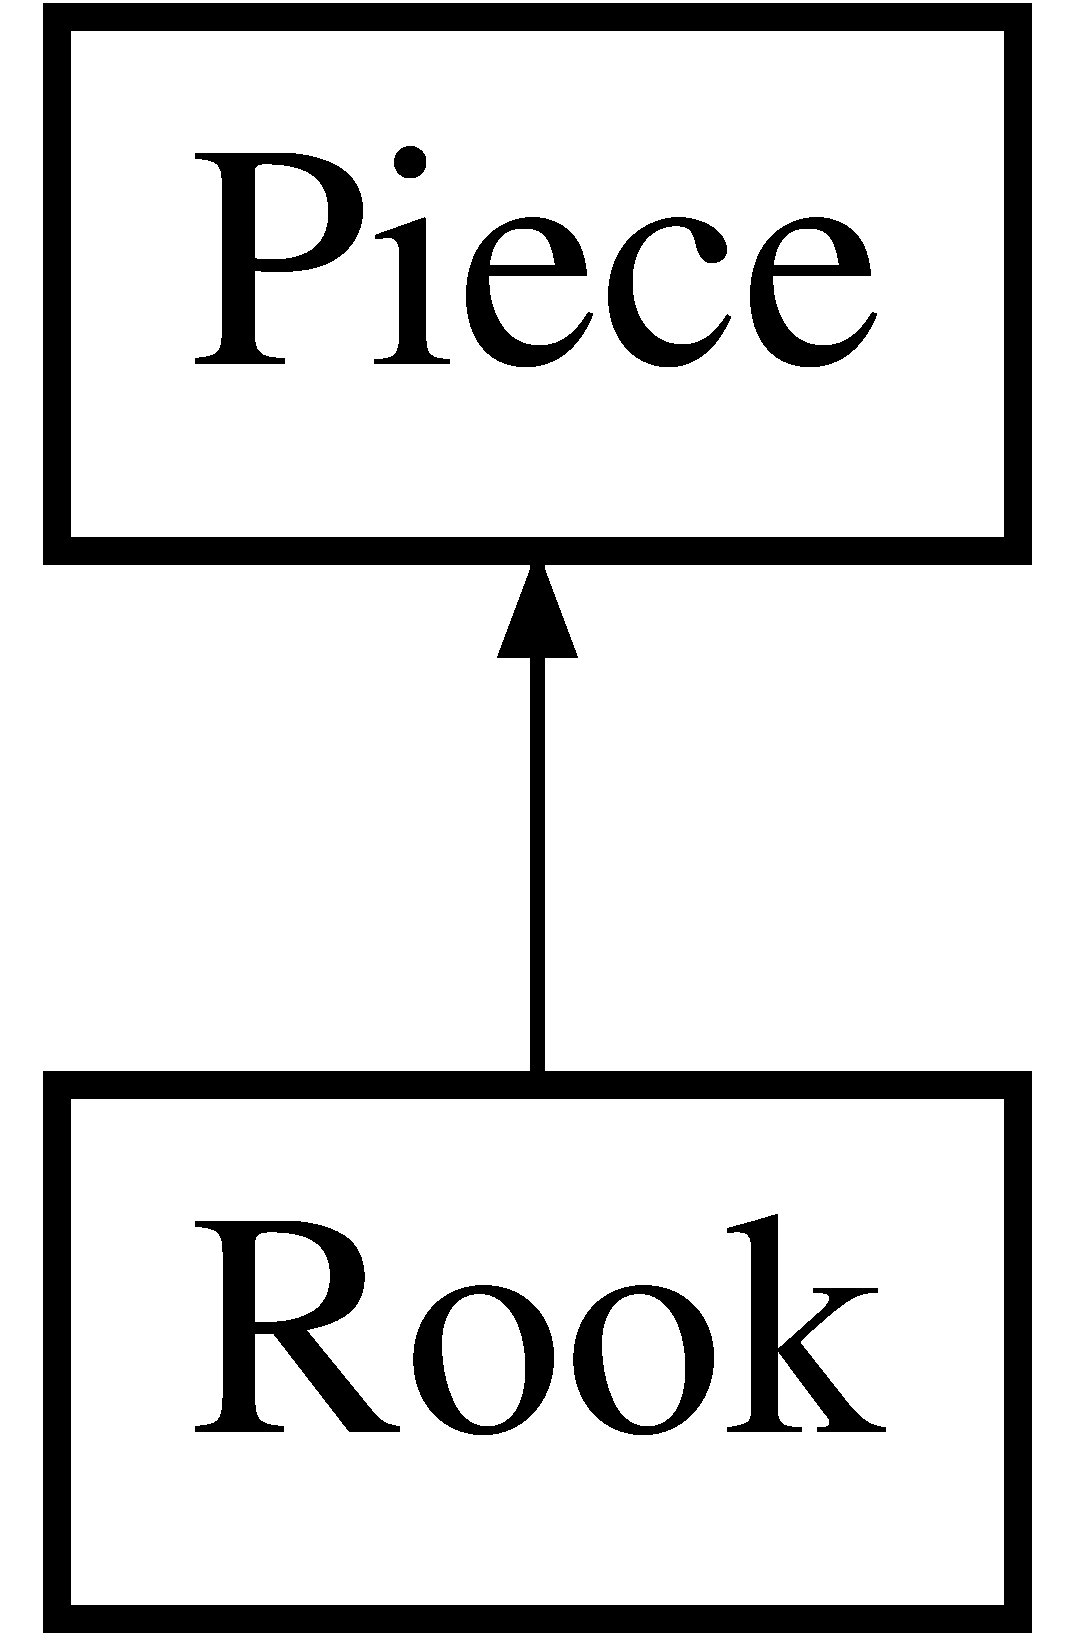
\includegraphics[height=2.000000cm]{class_rook}
\end{center}
\end{figure}
\subsection*{Public Member Functions}
\begin{DoxyCompactItemize}
\item 
\hyperlink{class_rook_a0cce560130c640f82c99937ce5781ac1}{Rook} ()
\item 
\hyperlink{class_rook_a5bb2e3899dc49bd53ba8428be36cc153}{Rook} (string \hyperlink{class_piece_a1b93d0ecc14e15fc7f3fb5def518502a}{position})
\item 
virtual \hyperlink{class_rook_a70d445b94848b22ded850b6f58bc2972}{$\sim$\+Rook} ()
\item 
vector$<$ string $>$ \hyperlink{class_rook_a96e1e49295f230cda98007a7df6d65fa}{get\+Avail\+Positions} (\hyperlink{class_piece}{Piece} $\ast$$\ast$all)
\end{DoxyCompactItemize}
\subsection*{Additional Inherited Members}


\subsection{Detailed Description}


Definition at line 18 of file Rook.\+h.



\subsection{Constructor \& Destructor Documentation}
\index{Rook@{Rook}!Rook@{Rook}}
\index{Rook@{Rook}!Rook@{Rook}}
\subsubsection[{\texorpdfstring{Rook()}{Rook()}}]{\setlength{\rightskip}{0pt plus 5cm}Rook\+::\+Rook (
\begin{DoxyParamCaption}
{}
\end{DoxyParamCaption}
)}\hypertarget{class_rook_a0cce560130c640f82c99937ce5781ac1}{}\label{class_rook_a0cce560130c640f82c99937ce5781ac1}
\index{Rook@{Rook}!Rook@{Rook}}
\index{Rook@{Rook}!Rook@{Rook}}
\subsubsection[{\texorpdfstring{Rook(string position)}{Rook(string position)}}]{\setlength{\rightskip}{0pt plus 5cm}Rook\+::\+Rook (
\begin{DoxyParamCaption}
\item[{string}]{position}
\end{DoxyParamCaption}
)\hspace{0.3cm}{\ttfamily [inline]}}\hypertarget{class_rook_a5bb2e3899dc49bd53ba8428be36cc153}{}\label{class_rook_a5bb2e3899dc49bd53ba8428be36cc153}


Definition at line 22 of file Rook.\+h.

\index{Rook@{Rook}!````~Rook@{$\sim$\+Rook}}
\index{````~Rook@{$\sim$\+Rook}!Rook@{Rook}}
\subsubsection[{\texorpdfstring{$\sim$\+Rook()}{~Rook()}}]{\setlength{\rightskip}{0pt plus 5cm}Rook\+::$\sim$\+Rook (
\begin{DoxyParamCaption}
{}
\end{DoxyParamCaption}
)\hspace{0.3cm}{\ttfamily [virtual]}}\hypertarget{class_rook_a70d445b94848b22ded850b6f58bc2972}{}\label{class_rook_a70d445b94848b22ded850b6f58bc2972}


Definition at line 11 of file Rook.\+cpp.



\subsection{Member Function Documentation}
\index{Rook@{Rook}!get\+Avail\+Positions@{get\+Avail\+Positions}}
\index{get\+Avail\+Positions@{get\+Avail\+Positions}!Rook@{Rook}}
\subsubsection[{\texorpdfstring{get\+Avail\+Positions(\+Piece $\ast$$\ast$all)}{getAvailPositions(Piece **all)}}]{\setlength{\rightskip}{0pt plus 5cm}vector$<$string$>$ Rook\+::get\+Avail\+Positions (
\begin{DoxyParamCaption}
\item[{{\bf Piece} $\ast$$\ast$}]{all}
\end{DoxyParamCaption}
)\hspace{0.3cm}{\ttfamily [inline]}, {\ttfamily [virtual]}}\hypertarget{class_rook_a96e1e49295f230cda98007a7df6d65fa}{}\label{class_rook_a96e1e49295f230cda98007a7df6d65fa}


Implements \hyperlink{class_piece_a4c717dfd8c910e2088bee2c4c6792c10}{Piece}.



Definition at line 28 of file Rook.\+h.



The documentation for this class was generated from the following files\+:\begin{DoxyCompactItemize}
\item 
\hyperlink{_rook_8h}{Rook.\+h}\item 
\hyperlink{_rook_8cpp}{Rook.\+cpp}\end{DoxyCompactItemize}

\chapter{File Documentation}
\hypertarget{_8dep_8inc}{}\section{.dep.\+inc File Reference}
\label{_8dep_8inc}\index{.\+dep.\+inc@{.\+dep.\+inc}}

\hypertarget{_bishop_8cpp}{}\section{Bishop.\+cpp File Reference}
\label{_bishop_8cpp}\index{Bishop.\+cpp@{Bishop.\+cpp}}
{\ttfamily \#include \char`\"{}Bishop.\+h\char`\"{}}\\*

\hypertarget{_bishop_8h}{}\section{Bishop.\+h File Reference}
\label{_bishop_8h}\index{Bishop.\+h@{Bishop.\+h}}
{\ttfamily \#include $<$string$>$}\\*
{\ttfamily \#include \char`\"{}Piece.\+h\char`\"{}}\\*
\subsection*{Classes}
\begin{DoxyCompactItemize}
\item 
class \hyperlink{class_bishop}{Bishop}
\end{DoxyCompactItemize}

\hypertarget{_cygwin-_windows_2_bishop_8o_8d}{}\section{build/\+Debug/\+Cygwin-\/\+Windows/\+Bishop.o.\+d File Reference}
\label{_cygwin-_windows_2_bishop_8o_8d}\index{build/\+Debug/\+Cygwin-\/\+Windows/\+Bishop.\+o.\+d@{build/\+Debug/\+Cygwin-\/\+Windows/\+Bishop.\+o.\+d}}

\hypertarget{_g_n_u-_linux_2_bishop_8o_8d}{}\section{build/\+Debug/\+G\+N\+U-\/\+Linux/\+Bishop.o.\+d File Reference}
\label{_g_n_u-_linux_2_bishop_8o_8d}\index{build/\+Debug/\+G\+N\+U-\/\+Linux/\+Bishop.\+o.\+d@{build/\+Debug/\+G\+N\+U-\/\+Linux/\+Bishop.\+o.\+d}}

\hypertarget{_cygwin-_windows_2_king_8o_8d}{}\section{build/\+Debug/\+Cygwin-\/\+Windows/\+King.o.\+d File Reference}
\label{_cygwin-_windows_2_king_8o_8d}\index{build/\+Debug/\+Cygwin-\/\+Windows/\+King.\+o.\+d@{build/\+Debug/\+Cygwin-\/\+Windows/\+King.\+o.\+d}}

\hypertarget{_g_n_u-_linux_2_king_8o_8d}{}\section{build/\+Debug/\+G\+N\+U-\/\+Linux/\+King.o.\+d File Reference}
\label{_g_n_u-_linux_2_king_8o_8d}\index{build/\+Debug/\+G\+N\+U-\/\+Linux/\+King.\+o.\+d@{build/\+Debug/\+G\+N\+U-\/\+Linux/\+King.\+o.\+d}}

\hypertarget{_cygwin-_windows_2_knight_8o_8d}{}\section{build/\+Debug/\+Cygwin-\/\+Windows/\+Knight.o.\+d File Reference}
\label{_cygwin-_windows_2_knight_8o_8d}\index{build/\+Debug/\+Cygwin-\/\+Windows/\+Knight.\+o.\+d@{build/\+Debug/\+Cygwin-\/\+Windows/\+Knight.\+o.\+d}}

\hypertarget{_g_n_u-_linux_2_knight_8o_8d}{}\section{build/\+Debug/\+G\+N\+U-\/\+Linux/\+Knight.o.\+d File Reference}
\label{_g_n_u-_linux_2_knight_8o_8d}\index{build/\+Debug/\+G\+N\+U-\/\+Linux/\+Knight.\+o.\+d@{build/\+Debug/\+G\+N\+U-\/\+Linux/\+Knight.\+o.\+d}}

\hypertarget{_cygwin-_windows_2main_8o_8d}{}\section{build/\+Debug/\+Cygwin-\/\+Windows/main.o.\+d File Reference}
\label{_cygwin-_windows_2main_8o_8d}\index{build/\+Debug/\+Cygwin-\/\+Windows/main.\+o.\+d@{build/\+Debug/\+Cygwin-\/\+Windows/main.\+o.\+d}}

\hypertarget{_g_n_u-_linux_2main_8o_8d}{}\section{build/\+Debug/\+G\+N\+U-\/\+Linux/main.o.\+d File Reference}
\label{_g_n_u-_linux_2main_8o_8d}\index{build/\+Debug/\+G\+N\+U-\/\+Linux/main.\+o.\+d@{build/\+Debug/\+G\+N\+U-\/\+Linux/main.\+o.\+d}}

\hypertarget{_cygwin-_windows_2_pawn_8o_8d}{}\section{build/\+Debug/\+Cygwin-\/\+Windows/\+Pawn.o.\+d File Reference}
\label{_cygwin-_windows_2_pawn_8o_8d}\index{build/\+Debug/\+Cygwin-\/\+Windows/\+Pawn.\+o.\+d@{build/\+Debug/\+Cygwin-\/\+Windows/\+Pawn.\+o.\+d}}

\hypertarget{_g_n_u-_linux_2_pawn_8o_8d}{}\section{build/\+Debug/\+G\+N\+U-\/\+Linux/\+Pawn.o.\+d File Reference}
\label{_g_n_u-_linux_2_pawn_8o_8d}\index{build/\+Debug/\+G\+N\+U-\/\+Linux/\+Pawn.\+o.\+d@{build/\+Debug/\+G\+N\+U-\/\+Linux/\+Pawn.\+o.\+d}}

\hypertarget{_cygwin-_windows_2_piece_8o_8d}{}\section{build/\+Debug/\+Cygwin-\/\+Windows/\+Piece.o.\+d File Reference}
\label{_cygwin-_windows_2_piece_8o_8d}\index{build/\+Debug/\+Cygwin-\/\+Windows/\+Piece.\+o.\+d@{build/\+Debug/\+Cygwin-\/\+Windows/\+Piece.\+o.\+d}}

\hypertarget{_g_n_u-_linux_2_piece_8o_8d}{}\section{build/\+Debug/\+G\+N\+U-\/\+Linux/\+Piece.o.\+d File Reference}
\label{_g_n_u-_linux_2_piece_8o_8d}\index{build/\+Debug/\+G\+N\+U-\/\+Linux/\+Piece.\+o.\+d@{build/\+Debug/\+G\+N\+U-\/\+Linux/\+Piece.\+o.\+d}}

\hypertarget{_cygwin-_windows_2_queen_8o_8d}{}\section{build/\+Debug/\+Cygwin-\/\+Windows/\+Queen.o.\+d File Reference}
\label{_cygwin-_windows_2_queen_8o_8d}\index{build/\+Debug/\+Cygwin-\/\+Windows/\+Queen.\+o.\+d@{build/\+Debug/\+Cygwin-\/\+Windows/\+Queen.\+o.\+d}}

\hypertarget{_g_n_u-_linux_2_queen_8o_8d}{}\section{build/\+Debug/\+G\+N\+U-\/\+Linux/\+Queen.o.\+d File Reference}
\label{_g_n_u-_linux_2_queen_8o_8d}\index{build/\+Debug/\+G\+N\+U-\/\+Linux/\+Queen.\+o.\+d@{build/\+Debug/\+G\+N\+U-\/\+Linux/\+Queen.\+o.\+d}}

\hypertarget{_cygwin-_windows_2_rook_8o_8d}{}\section{build/\+Debug/\+Cygwin-\/\+Windows/\+Rook.o.\+d File Reference}
\label{_cygwin-_windows_2_rook_8o_8d}\index{build/\+Debug/\+Cygwin-\/\+Windows/\+Rook.\+o.\+d@{build/\+Debug/\+Cygwin-\/\+Windows/\+Rook.\+o.\+d}}

\hypertarget{_g_n_u-_linux_2_rook_8o_8d}{}\section{build/\+Debug/\+G\+N\+U-\/\+Linux/\+Rook.o.\+d File Reference}
\label{_g_n_u-_linux_2_rook_8o_8d}\index{build/\+Debug/\+G\+N\+U-\/\+Linux/\+Rook.\+o.\+d@{build/\+Debug/\+G\+N\+U-\/\+Linux/\+Rook.\+o.\+d}}

\hypertarget{_colors_8h}{}\section{Colors.\+h File Reference}
\label{_colors_8h}\index{Colors.\+h@{Colors.\+h}}
\subsection*{Macros}
\begin{DoxyCompactItemize}
\item 
\#define \hyperlink{_colors_8h_ab702106cf3b3e96750b6845ded4e0299}{R\+E\+S\+ET}~\char`\"{}\textbackslash{}033\mbox{[}0m\char`\"{}
\item 
\#define \hyperlink{_colors_8h_a7b3b25cba33b07c303f3060fe41887f6}{B\+L\+A\+CK}~\char`\"{}\textbackslash{}033\mbox{[}30m\char`\"{}      /$\ast$ Black $\ast$/
\item 
\#define \hyperlink{_colors_8h_a8d23feea868a983c8c2b661e1e16972f}{R\+ED}~\char`\"{}\textbackslash{}033\mbox{[}31m\char`\"{}      /$\ast$ Red $\ast$/
\item 
\#define \hyperlink{_colors_8h_acfbc006ea433ad708fdee3e82996e721}{G\+R\+E\+EN}~\char`\"{}\textbackslash{}033\mbox{[}32m\char`\"{}      /$\ast$ Green $\ast$/
\item 
\#define \hyperlink{_colors_8h_abf681265909adf3d3e8116c93c0ba179}{Y\+E\+L\+L\+OW}~\char`\"{}\textbackslash{}033\mbox{[}33m\char`\"{}      /$\ast$ Yellow $\ast$/
\item 
\#define \hyperlink{_colors_8h_a79d10e672abb49ad63eeaa8aaef57c38}{B\+L\+UE}~\char`\"{}\textbackslash{}033\mbox{[}34m\char`\"{}      /$\ast$ Blue $\ast$/
\item 
\#define \hyperlink{_colors_8h_a6f699060902f800f12aaae150f3a708e}{M\+A\+G\+E\+N\+TA}~\char`\"{}\textbackslash{}033\mbox{[}35m\char`\"{}      /$\ast$ Magenta $\ast$/
\item 
\#define \hyperlink{_colors_8h_ad243f93c16bc4c1d3e0a13b84421d760}{C\+Y\+AN}~\char`\"{}\textbackslash{}033\mbox{[}36m\char`\"{}      /$\ast$ Cyan $\ast$/
\item 
\#define \hyperlink{_colors_8h_a87b537f5fa5c109d3c05c13d6b18f382}{W\+H\+I\+TE}~\char`\"{}\textbackslash{}033\mbox{[}37m\char`\"{}      /$\ast$ White $\ast$/
\item 
\#define \hyperlink{_colors_8h_aef2fe95894117165b29036718221979f}{B\+O\+L\+D\+B\+L\+A\+CK}~\char`\"{}\textbackslash{}033\mbox{[}1m\textbackslash{}033\mbox{[}30m\char`\"{}      /$\ast$ Bold Black $\ast$/
\item 
\#define \hyperlink{_colors_8h_ab912d02c7998c3d47d05f87be4e2c920}{B\+O\+L\+D\+R\+ED}~\char`\"{}\textbackslash{}033\mbox{[}1m\textbackslash{}033\mbox{[}31m\char`\"{}      /$\ast$ Bold Red $\ast$/
\item 
\#define \hyperlink{_colors_8h_a4a6c893a1703c33ede7d702fe5f97c91}{B\+O\+L\+D\+G\+R\+E\+EN}~\char`\"{}\textbackslash{}033\mbox{[}1m\textbackslash{}033\mbox{[}32m\char`\"{}      /$\ast$ Bold Green $\ast$/
\item 
\#define \hyperlink{_colors_8h_a8cec79108dfc3c61e8e32d390ec28b26}{B\+O\+L\+D\+Y\+E\+L\+L\+OW}~\char`\"{}\textbackslash{}033\mbox{[}1m\textbackslash{}033\mbox{[}33m\char`\"{}      /$\ast$ Bold Yellow $\ast$/
\item 
\#define \hyperlink{_colors_8h_a11e77c19555cbd15bcc744ff36a18635}{B\+O\+L\+D\+B\+L\+UE}~\char`\"{}\textbackslash{}033\mbox{[}1m\textbackslash{}033\mbox{[}34m\char`\"{}      /$\ast$ Bold Blue $\ast$/
\item 
\#define \hyperlink{_colors_8h_ac4723c5ee12cfca16e2172b57b99cb07}{B\+O\+L\+D\+M\+A\+G\+E\+N\+TA}~\char`\"{}\textbackslash{}033\mbox{[}1m\textbackslash{}033\mbox{[}35m\char`\"{}      /$\ast$ Bold Magenta $\ast$/
\item 
\#define \hyperlink{_colors_8h_ae87af5e6363eb1913b17f24dcb60a22d}{B\+O\+L\+D\+C\+Y\+AN}~\char`\"{}\textbackslash{}033\mbox{[}1m\textbackslash{}033\mbox{[}36m\char`\"{}      /$\ast$ Bold Cyan $\ast$/
\item 
\#define \hyperlink{_colors_8h_aa4ef051614aa0bd503b0a18ee158c5d7}{B\+O\+L\+D\+W\+H\+I\+TE}~\char`\"{}\textbackslash{}033\mbox{[}1m\textbackslash{}033\mbox{[}37m\char`\"{}      /$\ast$ Bold White $\ast$/
\item 
\#define \hyperlink{_colors_8h_ade269cc47cfaba70068f2586e898051d}{I\+N\+V\+E\+R\+SE}~\char`\"{}\textbackslash{}033\mbox{[}7m\char`\"{}     /$\ast$ Swap Bacground and Text colors $\ast$/
\item 
\#define \hyperlink{_colors_8h_aaec1a65734e33bc49e8dc8d90e9546bc}{U\+N\+D\+E\+R\+L\+I\+NE}~\char`\"{}\textbackslash{}033\mbox{[}4m\char`\"{}     /$\ast$ Underline Single $\ast$/
\item 
\#define \hyperlink{_colors_8h_ab4724fec8e2574110f93d0cebf25ac92}{B\+G\+B\+L\+A\+CK}~\char`\"{}\textbackslash{}033\mbox{[}40m\char`\"{}      /$\ast$ B\+L\+A\+C\+K Background $\ast$/
\item 
\#define \hyperlink{_colors_8h_a95e0a3871c4ee628ff78494e0c4e459a}{B\+G\+R\+ED}~\char`\"{}\textbackslash{}033\mbox{[}41m\char`\"{}      /$\ast$ R\+E\+D Background $\ast$/
\item 
\#define \hyperlink{_colors_8h_a898cbb3b8ecef2510cb6152b1f96d4c8}{B\+G\+G\+R\+E\+EN}~\char`\"{}\textbackslash{}033\mbox{[}42m\char`\"{}      /$\ast$ G\+R\+E\+E\+N Background $\ast$/
\item 
\#define \hyperlink{_colors_8h_ab68b1d2fc1f910b83d749ffa0a9a37f8}{B\+G\+Y\+E\+L\+L\+OW}~\char`\"{}\textbackslash{}033\mbox{[}43m\char`\"{}      /$\ast$ Y\+E\+L\+L\+O\+W Background $\ast$/
\item 
\#define \hyperlink{_colors_8h_a2c546b464622d186d669cfd8a4fa2947}{B\+G\+B\+L\+UE}~\char`\"{}\textbackslash{}033\mbox{[}44m\char`\"{}      /$\ast$ B\+L\+U\+E Background $\ast$/
\item 
\#define \hyperlink{_colors_8h_a96a8e22829e03241b315f0e8b34b49ad}{B\+G\+M\+A\+G\+E\+N\+TA}~\char`\"{}\textbackslash{}033\mbox{[}45m\char`\"{}      /$\ast$ M\+A\+G\+E\+N\+T\+A Background $\ast$/
\item 
\#define \hyperlink{_colors_8h_ade07cf7b38b0c36751e9c9880cb8792c}{B\+G\+C\+Y\+AN}~\char`\"{}\textbackslash{}033\mbox{[}46m\char`\"{}      /$\ast$ C\+Y\+A\+N Background $\ast$/
\item 
\#define \hyperlink{_colors_8h_ac7aa010e8e3ad6bbf4c725e52ba02168}{B\+G\+W\+H\+I\+TE}~\char`\"{}\textbackslash{}033\mbox{[}47m\char`\"{}      /$\ast$ W\+H\+I\+T\+E Background $\ast$/
\end{DoxyCompactItemize}


\subsection{Macro Definition Documentation}
\index{Colors.\+h@{Colors.\+h}!B\+G\+B\+L\+A\+CK@{B\+G\+B\+L\+A\+CK}}
\index{B\+G\+B\+L\+A\+CK@{B\+G\+B\+L\+A\+CK}!Colors.\+h@{Colors.\+h}}
\subsubsection[{\texorpdfstring{B\+G\+B\+L\+A\+CK}{BGBLACK}}]{\setlength{\rightskip}{0pt plus 5cm}\#define B\+G\+B\+L\+A\+CK~\char`\"{}\textbackslash{}033\mbox{[}40m\char`\"{}      /$\ast$ B\+L\+A\+C\+K Background $\ast$/}\hypertarget{_colors_8h_ab4724fec8e2574110f93d0cebf25ac92}{}\label{_colors_8h_ab4724fec8e2574110f93d0cebf25ac92}


Definition at line 33 of file Colors.\+h.

\index{Colors.\+h@{Colors.\+h}!B\+G\+B\+L\+UE@{B\+G\+B\+L\+UE}}
\index{B\+G\+B\+L\+UE@{B\+G\+B\+L\+UE}!Colors.\+h@{Colors.\+h}}
\subsubsection[{\texorpdfstring{B\+G\+B\+L\+UE}{BGBLUE}}]{\setlength{\rightskip}{0pt plus 5cm}\#define B\+G\+B\+L\+UE~\char`\"{}\textbackslash{}033\mbox{[}44m\char`\"{}      /$\ast$ B\+L\+U\+E Background $\ast$/}\hypertarget{_colors_8h_a2c546b464622d186d669cfd8a4fa2947}{}\label{_colors_8h_a2c546b464622d186d669cfd8a4fa2947}


Definition at line 37 of file Colors.\+h.

\index{Colors.\+h@{Colors.\+h}!B\+G\+C\+Y\+AN@{B\+G\+C\+Y\+AN}}
\index{B\+G\+C\+Y\+AN@{B\+G\+C\+Y\+AN}!Colors.\+h@{Colors.\+h}}
\subsubsection[{\texorpdfstring{B\+G\+C\+Y\+AN}{BGCYAN}}]{\setlength{\rightskip}{0pt plus 5cm}\#define B\+G\+C\+Y\+AN~\char`\"{}\textbackslash{}033\mbox{[}46m\char`\"{}      /$\ast$ C\+Y\+A\+N Background $\ast$/}\hypertarget{_colors_8h_ade07cf7b38b0c36751e9c9880cb8792c}{}\label{_colors_8h_ade07cf7b38b0c36751e9c9880cb8792c}


Definition at line 39 of file Colors.\+h.

\index{Colors.\+h@{Colors.\+h}!B\+G\+G\+R\+E\+EN@{B\+G\+G\+R\+E\+EN}}
\index{B\+G\+G\+R\+E\+EN@{B\+G\+G\+R\+E\+EN}!Colors.\+h@{Colors.\+h}}
\subsubsection[{\texorpdfstring{B\+G\+G\+R\+E\+EN}{BGGREEN}}]{\setlength{\rightskip}{0pt plus 5cm}\#define B\+G\+G\+R\+E\+EN~\char`\"{}\textbackslash{}033\mbox{[}42m\char`\"{}      /$\ast$ G\+R\+E\+E\+N Background $\ast$/}\hypertarget{_colors_8h_a898cbb3b8ecef2510cb6152b1f96d4c8}{}\label{_colors_8h_a898cbb3b8ecef2510cb6152b1f96d4c8}


Definition at line 35 of file Colors.\+h.

\index{Colors.\+h@{Colors.\+h}!B\+G\+M\+A\+G\+E\+N\+TA@{B\+G\+M\+A\+G\+E\+N\+TA}}
\index{B\+G\+M\+A\+G\+E\+N\+TA@{B\+G\+M\+A\+G\+E\+N\+TA}!Colors.\+h@{Colors.\+h}}
\subsubsection[{\texorpdfstring{B\+G\+M\+A\+G\+E\+N\+TA}{BGMAGENTA}}]{\setlength{\rightskip}{0pt plus 5cm}\#define B\+G\+M\+A\+G\+E\+N\+TA~\char`\"{}\textbackslash{}033\mbox{[}45m\char`\"{}      /$\ast$ M\+A\+G\+E\+N\+T\+A Background $\ast$/}\hypertarget{_colors_8h_a96a8e22829e03241b315f0e8b34b49ad}{}\label{_colors_8h_a96a8e22829e03241b315f0e8b34b49ad}


Definition at line 38 of file Colors.\+h.

\index{Colors.\+h@{Colors.\+h}!B\+G\+R\+ED@{B\+G\+R\+ED}}
\index{B\+G\+R\+ED@{B\+G\+R\+ED}!Colors.\+h@{Colors.\+h}}
\subsubsection[{\texorpdfstring{B\+G\+R\+ED}{BGRED}}]{\setlength{\rightskip}{0pt plus 5cm}\#define B\+G\+R\+ED~\char`\"{}\textbackslash{}033\mbox{[}41m\char`\"{}      /$\ast$ R\+E\+D Background $\ast$/}\hypertarget{_colors_8h_a95e0a3871c4ee628ff78494e0c4e459a}{}\label{_colors_8h_a95e0a3871c4ee628ff78494e0c4e459a}


Definition at line 34 of file Colors.\+h.

\index{Colors.\+h@{Colors.\+h}!B\+G\+W\+H\+I\+TE@{B\+G\+W\+H\+I\+TE}}
\index{B\+G\+W\+H\+I\+TE@{B\+G\+W\+H\+I\+TE}!Colors.\+h@{Colors.\+h}}
\subsubsection[{\texorpdfstring{B\+G\+W\+H\+I\+TE}{BGWHITE}}]{\setlength{\rightskip}{0pt plus 5cm}\#define B\+G\+W\+H\+I\+TE~\char`\"{}\textbackslash{}033\mbox{[}47m\char`\"{}      /$\ast$ W\+H\+I\+T\+E Background $\ast$/}\hypertarget{_colors_8h_ac7aa010e8e3ad6bbf4c725e52ba02168}{}\label{_colors_8h_ac7aa010e8e3ad6bbf4c725e52ba02168}


Definition at line 40 of file Colors.\+h.

\index{Colors.\+h@{Colors.\+h}!B\+G\+Y\+E\+L\+L\+OW@{B\+G\+Y\+E\+L\+L\+OW}}
\index{B\+G\+Y\+E\+L\+L\+OW@{B\+G\+Y\+E\+L\+L\+OW}!Colors.\+h@{Colors.\+h}}
\subsubsection[{\texorpdfstring{B\+G\+Y\+E\+L\+L\+OW}{BGYELLOW}}]{\setlength{\rightskip}{0pt plus 5cm}\#define B\+G\+Y\+E\+L\+L\+OW~\char`\"{}\textbackslash{}033\mbox{[}43m\char`\"{}      /$\ast$ Y\+E\+L\+L\+O\+W Background $\ast$/}\hypertarget{_colors_8h_ab68b1d2fc1f910b83d749ffa0a9a37f8}{}\label{_colors_8h_ab68b1d2fc1f910b83d749ffa0a9a37f8}


Definition at line 36 of file Colors.\+h.

\index{Colors.\+h@{Colors.\+h}!B\+L\+A\+CK@{B\+L\+A\+CK}}
\index{B\+L\+A\+CK@{B\+L\+A\+CK}!Colors.\+h@{Colors.\+h}}
\subsubsection[{\texorpdfstring{B\+L\+A\+CK}{BLACK}}]{\setlength{\rightskip}{0pt plus 5cm}\#define B\+L\+A\+CK~\char`\"{}\textbackslash{}033\mbox{[}30m\char`\"{}      /$\ast$ Black $\ast$/}\hypertarget{_colors_8h_a7b3b25cba33b07c303f3060fe41887f6}{}\label{_colors_8h_a7b3b25cba33b07c303f3060fe41887f6}


Definition at line 13 of file Colors.\+h.

\index{Colors.\+h@{Colors.\+h}!B\+L\+UE@{B\+L\+UE}}
\index{B\+L\+UE@{B\+L\+UE}!Colors.\+h@{Colors.\+h}}
\subsubsection[{\texorpdfstring{B\+L\+UE}{BLUE}}]{\setlength{\rightskip}{0pt plus 5cm}\#define B\+L\+UE~\char`\"{}\textbackslash{}033\mbox{[}34m\char`\"{}      /$\ast$ Blue $\ast$/}\hypertarget{_colors_8h_a79d10e672abb49ad63eeaa8aaef57c38}{}\label{_colors_8h_a79d10e672abb49ad63eeaa8aaef57c38}


Definition at line 17 of file Colors.\+h.

\index{Colors.\+h@{Colors.\+h}!B\+O\+L\+D\+B\+L\+A\+CK@{B\+O\+L\+D\+B\+L\+A\+CK}}
\index{B\+O\+L\+D\+B\+L\+A\+CK@{B\+O\+L\+D\+B\+L\+A\+CK}!Colors.\+h@{Colors.\+h}}
\subsubsection[{\texorpdfstring{B\+O\+L\+D\+B\+L\+A\+CK}{BOLDBLACK}}]{\setlength{\rightskip}{0pt plus 5cm}\#define B\+O\+L\+D\+B\+L\+A\+CK~\char`\"{}\textbackslash{}033\mbox{[}1m\textbackslash{}033\mbox{[}30m\char`\"{}      /$\ast$ Bold Black $\ast$/}\hypertarget{_colors_8h_aef2fe95894117165b29036718221979f}{}\label{_colors_8h_aef2fe95894117165b29036718221979f}


Definition at line 21 of file Colors.\+h.

\index{Colors.\+h@{Colors.\+h}!B\+O\+L\+D\+B\+L\+UE@{B\+O\+L\+D\+B\+L\+UE}}
\index{B\+O\+L\+D\+B\+L\+UE@{B\+O\+L\+D\+B\+L\+UE}!Colors.\+h@{Colors.\+h}}
\subsubsection[{\texorpdfstring{B\+O\+L\+D\+B\+L\+UE}{BOLDBLUE}}]{\setlength{\rightskip}{0pt plus 5cm}\#define B\+O\+L\+D\+B\+L\+UE~\char`\"{}\textbackslash{}033\mbox{[}1m\textbackslash{}033\mbox{[}34m\char`\"{}      /$\ast$ Bold Blue $\ast$/}\hypertarget{_colors_8h_a11e77c19555cbd15bcc744ff36a18635}{}\label{_colors_8h_a11e77c19555cbd15bcc744ff36a18635}


Definition at line 25 of file Colors.\+h.

\index{Colors.\+h@{Colors.\+h}!B\+O\+L\+D\+C\+Y\+AN@{B\+O\+L\+D\+C\+Y\+AN}}
\index{B\+O\+L\+D\+C\+Y\+AN@{B\+O\+L\+D\+C\+Y\+AN}!Colors.\+h@{Colors.\+h}}
\subsubsection[{\texorpdfstring{B\+O\+L\+D\+C\+Y\+AN}{BOLDCYAN}}]{\setlength{\rightskip}{0pt plus 5cm}\#define B\+O\+L\+D\+C\+Y\+AN~\char`\"{}\textbackslash{}033\mbox{[}1m\textbackslash{}033\mbox{[}36m\char`\"{}      /$\ast$ Bold Cyan $\ast$/}\hypertarget{_colors_8h_ae87af5e6363eb1913b17f24dcb60a22d}{}\label{_colors_8h_ae87af5e6363eb1913b17f24dcb60a22d}


Definition at line 27 of file Colors.\+h.

\index{Colors.\+h@{Colors.\+h}!B\+O\+L\+D\+G\+R\+E\+EN@{B\+O\+L\+D\+G\+R\+E\+EN}}
\index{B\+O\+L\+D\+G\+R\+E\+EN@{B\+O\+L\+D\+G\+R\+E\+EN}!Colors.\+h@{Colors.\+h}}
\subsubsection[{\texorpdfstring{B\+O\+L\+D\+G\+R\+E\+EN}{BOLDGREEN}}]{\setlength{\rightskip}{0pt plus 5cm}\#define B\+O\+L\+D\+G\+R\+E\+EN~\char`\"{}\textbackslash{}033\mbox{[}1m\textbackslash{}033\mbox{[}32m\char`\"{}      /$\ast$ Bold Green $\ast$/}\hypertarget{_colors_8h_a4a6c893a1703c33ede7d702fe5f97c91}{}\label{_colors_8h_a4a6c893a1703c33ede7d702fe5f97c91}


Definition at line 23 of file Colors.\+h.

\index{Colors.\+h@{Colors.\+h}!B\+O\+L\+D\+M\+A\+G\+E\+N\+TA@{B\+O\+L\+D\+M\+A\+G\+E\+N\+TA}}
\index{B\+O\+L\+D\+M\+A\+G\+E\+N\+TA@{B\+O\+L\+D\+M\+A\+G\+E\+N\+TA}!Colors.\+h@{Colors.\+h}}
\subsubsection[{\texorpdfstring{B\+O\+L\+D\+M\+A\+G\+E\+N\+TA}{BOLDMAGENTA}}]{\setlength{\rightskip}{0pt plus 5cm}\#define B\+O\+L\+D\+M\+A\+G\+E\+N\+TA~\char`\"{}\textbackslash{}033\mbox{[}1m\textbackslash{}033\mbox{[}35m\char`\"{}      /$\ast$ Bold Magenta $\ast$/}\hypertarget{_colors_8h_ac4723c5ee12cfca16e2172b57b99cb07}{}\label{_colors_8h_ac4723c5ee12cfca16e2172b57b99cb07}


Definition at line 26 of file Colors.\+h.

\index{Colors.\+h@{Colors.\+h}!B\+O\+L\+D\+R\+ED@{B\+O\+L\+D\+R\+ED}}
\index{B\+O\+L\+D\+R\+ED@{B\+O\+L\+D\+R\+ED}!Colors.\+h@{Colors.\+h}}
\subsubsection[{\texorpdfstring{B\+O\+L\+D\+R\+ED}{BOLDRED}}]{\setlength{\rightskip}{0pt plus 5cm}\#define B\+O\+L\+D\+R\+ED~\char`\"{}\textbackslash{}033\mbox{[}1m\textbackslash{}033\mbox{[}31m\char`\"{}      /$\ast$ Bold Red $\ast$/}\hypertarget{_colors_8h_ab912d02c7998c3d47d05f87be4e2c920}{}\label{_colors_8h_ab912d02c7998c3d47d05f87be4e2c920}


Definition at line 22 of file Colors.\+h.

\index{Colors.\+h@{Colors.\+h}!B\+O\+L\+D\+W\+H\+I\+TE@{B\+O\+L\+D\+W\+H\+I\+TE}}
\index{B\+O\+L\+D\+W\+H\+I\+TE@{B\+O\+L\+D\+W\+H\+I\+TE}!Colors.\+h@{Colors.\+h}}
\subsubsection[{\texorpdfstring{B\+O\+L\+D\+W\+H\+I\+TE}{BOLDWHITE}}]{\setlength{\rightskip}{0pt plus 5cm}\#define B\+O\+L\+D\+W\+H\+I\+TE~\char`\"{}\textbackslash{}033\mbox{[}1m\textbackslash{}033\mbox{[}37m\char`\"{}      /$\ast$ Bold White $\ast$/}\hypertarget{_colors_8h_aa4ef051614aa0bd503b0a18ee158c5d7}{}\label{_colors_8h_aa4ef051614aa0bd503b0a18ee158c5d7}


Definition at line 28 of file Colors.\+h.

\index{Colors.\+h@{Colors.\+h}!B\+O\+L\+D\+Y\+E\+L\+L\+OW@{B\+O\+L\+D\+Y\+E\+L\+L\+OW}}
\index{B\+O\+L\+D\+Y\+E\+L\+L\+OW@{B\+O\+L\+D\+Y\+E\+L\+L\+OW}!Colors.\+h@{Colors.\+h}}
\subsubsection[{\texorpdfstring{B\+O\+L\+D\+Y\+E\+L\+L\+OW}{BOLDYELLOW}}]{\setlength{\rightskip}{0pt plus 5cm}\#define B\+O\+L\+D\+Y\+E\+L\+L\+OW~\char`\"{}\textbackslash{}033\mbox{[}1m\textbackslash{}033\mbox{[}33m\char`\"{}      /$\ast$ Bold Yellow $\ast$/}\hypertarget{_colors_8h_a8cec79108dfc3c61e8e32d390ec28b26}{}\label{_colors_8h_a8cec79108dfc3c61e8e32d390ec28b26}


Definition at line 24 of file Colors.\+h.

\index{Colors.\+h@{Colors.\+h}!C\+Y\+AN@{C\+Y\+AN}}
\index{C\+Y\+AN@{C\+Y\+AN}!Colors.\+h@{Colors.\+h}}
\subsubsection[{\texorpdfstring{C\+Y\+AN}{CYAN}}]{\setlength{\rightskip}{0pt plus 5cm}\#define C\+Y\+AN~\char`\"{}\textbackslash{}033\mbox{[}36m\char`\"{}      /$\ast$ Cyan $\ast$/}\hypertarget{_colors_8h_ad243f93c16bc4c1d3e0a13b84421d760}{}\label{_colors_8h_ad243f93c16bc4c1d3e0a13b84421d760}


Definition at line 19 of file Colors.\+h.

\index{Colors.\+h@{Colors.\+h}!G\+R\+E\+EN@{G\+R\+E\+EN}}
\index{G\+R\+E\+EN@{G\+R\+E\+EN}!Colors.\+h@{Colors.\+h}}
\subsubsection[{\texorpdfstring{G\+R\+E\+EN}{GREEN}}]{\setlength{\rightskip}{0pt plus 5cm}\#define G\+R\+E\+EN~\char`\"{}\textbackslash{}033\mbox{[}32m\char`\"{}      /$\ast$ Green $\ast$/}\hypertarget{_colors_8h_acfbc006ea433ad708fdee3e82996e721}{}\label{_colors_8h_acfbc006ea433ad708fdee3e82996e721}


Definition at line 15 of file Colors.\+h.

\index{Colors.\+h@{Colors.\+h}!I\+N\+V\+E\+R\+SE@{I\+N\+V\+E\+R\+SE}}
\index{I\+N\+V\+E\+R\+SE@{I\+N\+V\+E\+R\+SE}!Colors.\+h@{Colors.\+h}}
\subsubsection[{\texorpdfstring{I\+N\+V\+E\+R\+SE}{INVERSE}}]{\setlength{\rightskip}{0pt plus 5cm}\#define I\+N\+V\+E\+R\+SE~\char`\"{}\textbackslash{}033\mbox{[}7m\char`\"{}     /$\ast$ Swap Bacground and Text colors $\ast$/}\hypertarget{_colors_8h_ade269cc47cfaba70068f2586e898051d}{}\label{_colors_8h_ade269cc47cfaba70068f2586e898051d}


Definition at line 30 of file Colors.\+h.

\index{Colors.\+h@{Colors.\+h}!M\+A\+G\+E\+N\+TA@{M\+A\+G\+E\+N\+TA}}
\index{M\+A\+G\+E\+N\+TA@{M\+A\+G\+E\+N\+TA}!Colors.\+h@{Colors.\+h}}
\subsubsection[{\texorpdfstring{M\+A\+G\+E\+N\+TA}{MAGENTA}}]{\setlength{\rightskip}{0pt plus 5cm}\#define M\+A\+G\+E\+N\+TA~\char`\"{}\textbackslash{}033\mbox{[}35m\char`\"{}      /$\ast$ Magenta $\ast$/}\hypertarget{_colors_8h_a6f699060902f800f12aaae150f3a708e}{}\label{_colors_8h_a6f699060902f800f12aaae150f3a708e}


Definition at line 18 of file Colors.\+h.

\index{Colors.\+h@{Colors.\+h}!R\+ED@{R\+ED}}
\index{R\+ED@{R\+ED}!Colors.\+h@{Colors.\+h}}
\subsubsection[{\texorpdfstring{R\+ED}{RED}}]{\setlength{\rightskip}{0pt plus 5cm}\#define R\+ED~\char`\"{}\textbackslash{}033\mbox{[}31m\char`\"{}      /$\ast$ Red $\ast$/}\hypertarget{_colors_8h_a8d23feea868a983c8c2b661e1e16972f}{}\label{_colors_8h_a8d23feea868a983c8c2b661e1e16972f}


Definition at line 14 of file Colors.\+h.

\index{Colors.\+h@{Colors.\+h}!R\+E\+S\+ET@{R\+E\+S\+ET}}
\index{R\+E\+S\+ET@{R\+E\+S\+ET}!Colors.\+h@{Colors.\+h}}
\subsubsection[{\texorpdfstring{R\+E\+S\+ET}{RESET}}]{\setlength{\rightskip}{0pt plus 5cm}\#define R\+E\+S\+ET~\char`\"{}\textbackslash{}033\mbox{[}0m\char`\"{}}\hypertarget{_colors_8h_ab702106cf3b3e96750b6845ded4e0299}{}\label{_colors_8h_ab702106cf3b3e96750b6845ded4e0299}


Definition at line 12 of file Colors.\+h.

\index{Colors.\+h@{Colors.\+h}!U\+N\+D\+E\+R\+L\+I\+NE@{U\+N\+D\+E\+R\+L\+I\+NE}}
\index{U\+N\+D\+E\+R\+L\+I\+NE@{U\+N\+D\+E\+R\+L\+I\+NE}!Colors.\+h@{Colors.\+h}}
\subsubsection[{\texorpdfstring{U\+N\+D\+E\+R\+L\+I\+NE}{UNDERLINE}}]{\setlength{\rightskip}{0pt plus 5cm}\#define U\+N\+D\+E\+R\+L\+I\+NE~\char`\"{}\textbackslash{}033\mbox{[}4m\char`\"{}     /$\ast$ Underline Single $\ast$/}\hypertarget{_colors_8h_aaec1a65734e33bc49e8dc8d90e9546bc}{}\label{_colors_8h_aaec1a65734e33bc49e8dc8d90e9546bc}


Definition at line 31 of file Colors.\+h.

\index{Colors.\+h@{Colors.\+h}!W\+H\+I\+TE@{W\+H\+I\+TE}}
\index{W\+H\+I\+TE@{W\+H\+I\+TE}!Colors.\+h@{Colors.\+h}}
\subsubsection[{\texorpdfstring{W\+H\+I\+TE}{WHITE}}]{\setlength{\rightskip}{0pt plus 5cm}\#define W\+H\+I\+TE~\char`\"{}\textbackslash{}033\mbox{[}37m\char`\"{}      /$\ast$ White $\ast$/}\hypertarget{_colors_8h_a87b537f5fa5c109d3c05c13d6b18f382}{}\label{_colors_8h_a87b537f5fa5c109d3c05c13d6b18f382}


Definition at line 20 of file Colors.\+h.

\index{Colors.\+h@{Colors.\+h}!Y\+E\+L\+L\+OW@{Y\+E\+L\+L\+OW}}
\index{Y\+E\+L\+L\+OW@{Y\+E\+L\+L\+OW}!Colors.\+h@{Colors.\+h}}
\subsubsection[{\texorpdfstring{Y\+E\+L\+L\+OW}{YELLOW}}]{\setlength{\rightskip}{0pt plus 5cm}\#define Y\+E\+L\+L\+OW~\char`\"{}\textbackslash{}033\mbox{[}33m\char`\"{}      /$\ast$ Yellow $\ast$/}\hypertarget{_colors_8h_abf681265909adf3d3e8116c93c0ba179}{}\label{_colors_8h_abf681265909adf3d3e8116c93c0ba179}


Definition at line 16 of file Colors.\+h.


\hypertarget{_king_8cpp}{}\section{King.\+cpp File Reference}
\label{_king_8cpp}\index{King.\+cpp@{King.\+cpp}}
{\ttfamily \#include \char`\"{}King.\+h\char`\"{}}\\*

\hypertarget{_king_8h}{}\section{King.\+h File Reference}
\label{_king_8h}\index{King.\+h@{King.\+h}}
{\ttfamily \#include $<$string$>$}\\*
{\ttfamily \#include \char`\"{}Piece.\+h\char`\"{}}\\*
\subsection*{Classes}
\begin{DoxyCompactItemize}
\item 
class \hyperlink{class_king}{King}
\end{DoxyCompactItemize}

\hypertarget{_knight_8cpp}{}\section{Knight.\+cpp File Reference}
\label{_knight_8cpp}\index{Knight.\+cpp@{Knight.\+cpp}}
{\ttfamily \#include \char`\"{}Knight.\+h\char`\"{}}\\*

\hypertarget{_knight_8h}{}\section{Knight.\+h File Reference}
\label{_knight_8h}\index{Knight.\+h@{Knight.\+h}}
{\ttfamily \#include $<$string$>$}\\*
{\ttfamily \#include \char`\"{}Piece.\+h\char`\"{}}\\*
\subsection*{Classes}
\begin{DoxyCompactItemize}
\item 
class \hyperlink{class_knight}{Knight}
\end{DoxyCompactItemize}

\hypertarget{main_8cpp}{}\section{main.\+cpp File Reference}
\label{main_8cpp}\index{main.\+cpp@{main.\+cpp}}
{\ttfamily \#include $<$cstdlib$>$}\\*
{\ttfamily \#include $<$iostream$>$}\\*
{\ttfamily \#include $<$iomanip$>$}\\*
{\ttfamily \#include $<$fstream$>$}\\*
{\ttfamily \#include $<$string$>$}\\*
{\ttfamily \#include $<$map$>$}\\*
{\ttfamily \#include $<$sstream$>$}\\*
{\ttfamily \#include $<$cctype$>$}\\*
{\ttfamily \#include $<$new$>$}\\*
{\ttfamily \#include $<$algorithm$>$}\\*
{\ttfamily \#include \char`\"{}Pawn.\+h\char`\"{}}\\*
{\ttfamily \#include \char`\"{}Knight.\+h\char`\"{}}\\*
{\ttfamily \#include \char`\"{}Bishop.\+h\char`\"{}}\\*
{\ttfamily \#include \char`\"{}Rook.\+h\char`\"{}}\\*
{\ttfamily \#include \char`\"{}King.\+h\char`\"{}}\\*
{\ttfamily \#include \char`\"{}Queen.\+h\char`\"{}}\\*
{\ttfamily \#include \char`\"{}Piece.\+h\char`\"{}}\\*
{\ttfamily \#include \char`\"{}Colors.\+h\char`\"{}}\\*
\subsection*{Functions}
\begin{DoxyCompactItemize}
\item 
void \hyperlink{main_8cpp_a6444331b153d596d89373aa8d7e0b59d}{init\+Coords} (map$<$ string, int $>$ \&m)
\item 
void \hyperlink{main_8cpp_acbb08b4dcc07e59a39127c08b173fcbd}{draw\+Board} (fstream \&new\+Game, short \&col)
\item 
void \hyperlink{main_8cpp_a460fb296898806fec6667a62a14676cb}{refresh\+Board} ()
\item 
void \hyperlink{main_8cpp_ae34c19d5c237a304314afd5ab91a8a2e}{set\+All\+Index} (\hyperlink{class_piece}{Piece} $\ast$$\ast$all, \hyperlink{class_piece}{Piece} $\ast$$\ast$type, short i, short index, short half)
\item 
void \hyperlink{main_8cpp_a7968a1ad5805e21a2719c066ab2bc386}{init\+Pieces} (\hyperlink{class_piece}{Piece} $\ast$$\ast$pawns, \hyperlink{class_piece}{Piece} $\ast$$\ast$knights, \hyperlink{class_piece}{Piece} $\ast$$\ast$bishops, \hyperlink{class_piece}{Piece} $\ast$$\ast$rooks, \hyperlink{class_piece}{Piece} $\ast$$\ast$kings, \hyperlink{class_piece}{Piece} $\ast$$\ast$queens, \hyperlink{class_piece}{Piece} $\ast$$\ast$all)
\item 
bool \hyperlink{main_8cpp_aa9694c3d590b73cbaecba769bebee7c5}{proceed} (\hyperlink{class_piece}{Piece} $\ast$$\ast$piece, \hyperlink{class_piece}{Piece} $\ast$$\ast$all, string \&input, short \&turn)
\item 
void \hyperlink{main_8cpp_a956389361790fe2c581a4634495acda1}{collect\+Input} (string \&input, string \&input2, \hyperlink{class_piece}{Piece} $\ast$$\ast$all, \hyperlink{class_piece}{Piece} $\ast$$\ast$piece, fstream \&f, map$<$ string, int $>$ \&m, short \&col, short \&turn, \hyperlink{class_piece}{Piece} $\ast$$\ast$kings)
\item 
void \hyperlink{main_8cpp_a710cff68311c045ceee4ccc30eae9ca6}{check4check} (\hyperlink{class_piece}{Piece} $\ast$$\ast$all, \hyperlink{class_piece}{Piece} $\ast$$\ast$kings)
\item 
void \hyperlink{main_8cpp_a2c0ed726348eabc1d0870f40aa356498}{clean\+Up} (\hyperlink{class_piece}{Piece} $\ast$$\ast$pawns, \hyperlink{class_piece}{Piece} $\ast$$\ast$knights, \hyperlink{class_piece}{Piece} $\ast$$\ast$bishops, \hyperlink{class_piece}{Piece} $\ast$$\ast$rooks, \hyperlink{class_piece}{Piece} $\ast$$\ast$kings, \hyperlink{class_piece}{Piece} $\ast$$\ast$queens, \hyperlink{class_piece}{Piece} $\ast$$\ast$all, \hyperlink{class_piece}{Piece} $\ast$$\ast$piece)
\item 
void \hyperlink{main_8cpp_a83634c8b8036d339c72a5fb026c238aa}{update\+Hints} (fstream \&f, vector$<$ string $>$ \&v, map$<$ string, int $>$ m, string val, bool print)
\item 
bool \hyperlink{main_8cpp_a908402886673f8a7a5dc4f54e6057602}{validate\+Input} (string \&input)
\item 
{\footnotesize template$<$class T $>$ }\\void \hyperlink{main_8cpp_aaed4f7a95c858511e4dc3f56995903b8}{init\+Piece} (\hyperlink{class_piece}{Piece} $\ast$$\ast$type, \hyperlink{class_piece}{Piece} $\ast$$\ast$all, short size)
\item 
{\footnotesize template$<$class T $>$ }\\void \hyperlink{main_8cpp_ad485d65fa04c45c00b5205f922ff7182}{init\+Piece} (\hyperlink{class_piece}{Piece} $\ast$$\ast$type, \hyperlink{class_piece}{Piece} $\ast$$\ast$all, short size, short a, short b, short index)
\item 
int \hyperlink{main_8cpp_a3c04138a5bfe5d72780bb7e82a18e627}{main} (int argc, char $\ast$$\ast$argv)
\end{DoxyCompactItemize}
\subsection*{Variables}
\begin{DoxyCompactItemize}
\item 
const string \hyperlink{main_8cpp_acec89b22d9ab6e6b45e9b90207a51a3b}{R\+E\+AD} = \char`\"{}newgame.\+txt\char`\"{}
\item 
const string \hyperlink{main_8cpp_a0541d25e3bd8e29cd68a0a0a26de76f1}{W\+R\+I\+TE} = \char`\"{}game.\+txt\char`\"{}
\end{DoxyCompactItemize}


\subsection{Function Documentation}
\index{main.\+cpp@{main.\+cpp}!check4check@{check4check}}
\index{check4check@{check4check}!main.\+cpp@{main.\+cpp}}
\subsubsection[{\texorpdfstring{check4check(\+Piece $\ast$$\ast$all, Piece $\ast$$\ast$kings)}{check4check(Piece **all, Piece **kings)}}]{\setlength{\rightskip}{0pt plus 5cm}void check4check (
\begin{DoxyParamCaption}
\item[{{\bf Piece} $\ast$$\ast$}]{all, }
\item[{{\bf Piece} $\ast$$\ast$}]{kings}
\end{DoxyParamCaption}
)}\hypertarget{main_8cpp_a710cff68311c045ceee4ccc30eae9ca6}{}\label{main_8cpp_a710cff68311c045ceee4ccc30eae9ca6}
Loop through all Pieces, then all Pieces\textquotesingle{} available\+Positions. See if a king is in check and print a message if so. 

Definition at line 330 of file main.\+cpp.

\index{main.\+cpp@{main.\+cpp}!clean\+Up@{clean\+Up}}
\index{clean\+Up@{clean\+Up}!main.\+cpp@{main.\+cpp}}
\subsubsection[{\texorpdfstring{clean\+Up(\+Piece $\ast$$\ast$pawns, Piece $\ast$$\ast$knights, Piece $\ast$$\ast$bishops, Piece $\ast$$\ast$rooks, Piece $\ast$$\ast$kings, Piece $\ast$$\ast$queens, Piece $\ast$$\ast$all, Piece $\ast$$\ast$piece)}{cleanUp(Piece **pawns, Piece **knights, Piece **bishops, Piece **rooks, Piece **kings, Piece **queens, Piece **all, Piece **piece)}}]{\setlength{\rightskip}{0pt plus 5cm}void clean\+Up (
\begin{DoxyParamCaption}
\item[{{\bf Piece} $\ast$$\ast$}]{pawns, }
\item[{{\bf Piece} $\ast$$\ast$}]{knights, }
\item[{{\bf Piece} $\ast$$\ast$}]{bishops, }
\item[{{\bf Piece} $\ast$$\ast$}]{rooks, }
\item[{{\bf Piece} $\ast$$\ast$}]{kings, }
\item[{{\bf Piece} $\ast$$\ast$}]{queens, }
\item[{{\bf Piece} $\ast$$\ast$}]{all, }
\item[{{\bf Piece} $\ast$$\ast$}]{piece}
\end{DoxyParamCaption}
)}\hypertarget{main_8cpp_a2c0ed726348eabc1d0870f40aa356498}{}\label{main_8cpp_a2c0ed726348eabc1d0870f40aa356498}
Delete and and clean all uses of dynamic memory. 

Definition at line 153 of file main.\+cpp.

\index{main.\+cpp@{main.\+cpp}!collect\+Input@{collect\+Input}}
\index{collect\+Input@{collect\+Input}!main.\+cpp@{main.\+cpp}}
\subsubsection[{\texorpdfstring{collect\+Input(string \&input, string \&input2, Piece $\ast$$\ast$all, Piece $\ast$$\ast$piece, fstream \&f, map$<$ string, int $>$ \&m, short \&col, short \&turn, Piece $\ast$$\ast$kings)}{collectInput(string &input, string &input2, Piece **all, Piece **piece, fstream &f, map< string, int > &m, short &col, short &turn, Piece **kings)}}]{\setlength{\rightskip}{0pt plus 5cm}void collect\+Input (
\begin{DoxyParamCaption}
\item[{string \&}]{input, }
\item[{string \&}]{input2, }
\item[{{\bf Piece} $\ast$$\ast$}]{all, }
\item[{{\bf Piece} $\ast$$\ast$}]{piece, }
\item[{fstream \&}]{f, }
\item[{map$<$ string, int $>$ \&}]{m, }
\item[{short \&}]{col, }
\item[{short \&}]{turn, }
\item[{{\bf Piece} $\ast$$\ast$}]{kings}
\end{DoxyParamCaption}
)}\hypertarget{main_8cpp_a956389361790fe2c581a4634495acda1}{}\label{main_8cpp_a956389361790fe2c581a4634495acda1}
Collect a target \hyperlink{class_piece}{Piece} to maneuver, then collect a destination square for that \hyperlink{class_piece}{Piece}. Update the Board, then process the next player\textquotesingle{}s turn. 

Definition at line 276 of file main.\+cpp.

\index{main.\+cpp@{main.\+cpp}!draw\+Board@{draw\+Board}}
\index{draw\+Board@{draw\+Board}!main.\+cpp@{main.\+cpp}}
\subsubsection[{\texorpdfstring{draw\+Board(fstream \&new\+Game, short \&col)}{drawBoard(fstream &newGame, short &col)}}]{\setlength{\rightskip}{0pt plus 5cm}void draw\+Board (
\begin{DoxyParamCaption}
\item[{fstream \&}]{new\+Game, }
\item[{short \&}]{col}
\end{DoxyParamCaption}
)}\hypertarget{main_8cpp_acbb08b4dcc07e59a39127c08b173fcbd}{}\label{main_8cpp_acbb08b4dcc07e59a39127c08b173fcbd}
Reads the Board from the game file and prints all characters onto the Board. Also displays A-\/H and 0-\/7 coordinate-\/system-\/\+UI 

Definition at line 422 of file main.\+cpp.

\index{main.\+cpp@{main.\+cpp}!init\+Coords@{init\+Coords}}
\index{init\+Coords@{init\+Coords}!main.\+cpp@{main.\+cpp}}
\subsubsection[{\texorpdfstring{init\+Coords(map$<$ string, int $>$ \&m)}{initCoords(map< string, int > &m)}}]{\setlength{\rightskip}{0pt plus 5cm}void init\+Coords (
\begin{DoxyParamCaption}
\item[{map$<$ string, int $>$ \&}]{m}
\end{DoxyParamCaption}
)}\hypertarget{main_8cpp_a6444331b153d596d89373aa8d7e0b59d}{}\label{main_8cpp_a6444331b153d596d89373aa8d7e0b59d}
Map the coordinates on the grid where the letters should appear for each grid square. A0 = square 1, H7 = square 64, representing an 8x8 grid. 

Definition at line 479 of file main.\+cpp.

\index{main.\+cpp@{main.\+cpp}!init\+Piece@{init\+Piece}}
\index{init\+Piece@{init\+Piece}!main.\+cpp@{main.\+cpp}}
\subsubsection[{\texorpdfstring{init\+Piece(\+Piece $\ast$$\ast$type, Piece $\ast$$\ast$all, short size)}{initPiece(Piece **type, Piece **all, short size)}}]{\setlength{\rightskip}{0pt plus 5cm}template$<$class T $>$ void init\+Piece (
\begin{DoxyParamCaption}
\item[{{\bf Piece} $\ast$$\ast$}]{type, }
\item[{{\bf Piece} $\ast$$\ast$}]{all, }
\item[{short}]{size}
\end{DoxyParamCaption}
)}\hypertarget{main_8cpp_aaed4f7a95c858511e4dc3f56995903b8}{}\label{main_8cpp_aaed4f7a95c858511e4dc3f56995903b8}
Initialize the Pawns 

Definition at line 68 of file main.\+cpp.

\index{main.\+cpp@{main.\+cpp}!init\+Piece@{init\+Piece}}
\index{init\+Piece@{init\+Piece}!main.\+cpp@{main.\+cpp}}
\subsubsection[{\texorpdfstring{init\+Piece(\+Piece $\ast$$\ast$type, Piece $\ast$$\ast$all, short size, short a, short b, short index)}{initPiece(Piece **type, Piece **all, short size, short a, short b, short index)}}]{\setlength{\rightskip}{0pt plus 5cm}template$<$class T $>$ void init\+Piece (
\begin{DoxyParamCaption}
\item[{{\bf Piece} $\ast$$\ast$}]{type, }
\item[{{\bf Piece} $\ast$$\ast$}]{all, }
\item[{short}]{size, }
\item[{short}]{a, }
\item[{short}]{b, }
\item[{short}]{index}
\end{DoxyParamCaption}
)}\hypertarget{main_8cpp_ad485d65fa04c45c00b5205f922ff7182}{}\label{main_8cpp_ad485d65fa04c45c00b5205f922ff7182}
Initialize the rest of the Pieces 

Definition at line 83 of file main.\+cpp.

\index{main.\+cpp@{main.\+cpp}!init\+Pieces@{init\+Pieces}}
\index{init\+Pieces@{init\+Pieces}!main.\+cpp@{main.\+cpp}}
\subsubsection[{\texorpdfstring{init\+Pieces(\+Piece $\ast$$\ast$pawns, Piece $\ast$$\ast$knights, Piece $\ast$$\ast$bishops, Piece $\ast$$\ast$rooks, Piece $\ast$$\ast$kings, Piece $\ast$$\ast$queens, Piece $\ast$$\ast$all)}{initPieces(Piece **pawns, Piece **knights, Piece **bishops, Piece **rooks, Piece **kings, Piece **queens, Piece **all)}}]{\setlength{\rightskip}{0pt plus 5cm}void init\+Pieces (
\begin{DoxyParamCaption}
\item[{{\bf Piece} $\ast$$\ast$}]{pawns, }
\item[{{\bf Piece} $\ast$$\ast$}]{knights, }
\item[{{\bf Piece} $\ast$$\ast$}]{bishops, }
\item[{{\bf Piece} $\ast$$\ast$}]{rooks, }
\item[{{\bf Piece} $\ast$$\ast$}]{kings, }
\item[{{\bf Piece} $\ast$$\ast$}]{queens, }
\item[{{\bf Piece} $\ast$$\ast$}]{all}
\end{DoxyParamCaption}
)}\hypertarget{main_8cpp_a7968a1ad5805e21a2719c066ab2bc386}{}\label{main_8cpp_a7968a1ad5805e21a2719c066ab2bc386}
Initialize all pieces in the arrays. 

Definition at line 386 of file main.\+cpp.

\index{main.\+cpp@{main.\+cpp}!main@{main}}
\index{main@{main}!main.\+cpp@{main.\+cpp}}
\subsubsection[{\texorpdfstring{main(int argc, char $\ast$$\ast$argv)}{main(int argc, char **argv)}}]{\setlength{\rightskip}{0pt plus 5cm}int main (
\begin{DoxyParamCaption}
\item[{int}]{argc, }
\item[{char $\ast$$\ast$}]{argv}
\end{DoxyParamCaption}
)}\hypertarget{main_8cpp_a3c04138a5bfe5d72780bb7e82a18e627}{}\label{main_8cpp_a3c04138a5bfe5d72780bb7e82a18e627}
Create the coordinate system. Clear the Board so that it is blank, then initialize Pieces in their starting positions. While-\/loop until a king has been captured, meanwhile collect input. When a king is captured, display who the loser of the game is. 

Definition at line 102 of file main.\+cpp.

\index{main.\+cpp@{main.\+cpp}!proceed@{proceed}}
\index{proceed@{proceed}!main.\+cpp@{main.\+cpp}}
\subsubsection[{\texorpdfstring{proceed(\+Piece $\ast$$\ast$piece, Piece $\ast$$\ast$all, string \&input, short \&turn)}{proceed(Piece **piece, Piece **all, string &input, short &turn)}}]{\setlength{\rightskip}{0pt plus 5cm}bool proceed (
\begin{DoxyParamCaption}
\item[{{\bf Piece} $\ast$$\ast$}]{piece, }
\item[{{\bf Piece} $\ast$$\ast$}]{all, }
\item[{string \&}]{input, }
\item[{short \&}]{turn}
\end{DoxyParamCaption}
)}\hypertarget{main_8cpp_aa9694c3d590b73cbaecba769bebee7c5}{}\label{main_8cpp_aa9694c3d590b73cbaecba769bebee7c5}
Collect the first input, that is, the \hyperlink{class_piece}{Piece} to maneuver. Exit early if the wrong player is taking a turn. 

Definition at line 230 of file main.\+cpp.

\index{main.\+cpp@{main.\+cpp}!refresh\+Board@{refresh\+Board}}
\index{refresh\+Board@{refresh\+Board}!main.\+cpp@{main.\+cpp}}
\subsubsection[{\texorpdfstring{refresh\+Board()}{refreshBoard()}}]{\setlength{\rightskip}{0pt plus 5cm}void refresh\+Board (
\begin{DoxyParamCaption}
{}
\end{DoxyParamCaption}
)}\hypertarget{main_8cpp_a460fb296898806fec6667a62a14676cb}{}\label{main_8cpp_a460fb296898806fec6667a62a14676cb}
Rewrite the board from a read-\/only file containing the blank map with no pieces. 

Definition at line 401 of file main.\+cpp.

\index{main.\+cpp@{main.\+cpp}!set\+All\+Index@{set\+All\+Index}}
\index{set\+All\+Index@{set\+All\+Index}!main.\+cpp@{main.\+cpp}}
\subsubsection[{\texorpdfstring{set\+All\+Index(\+Piece $\ast$$\ast$all, Piece $\ast$$\ast$type, short i, short index, short half)}{setAllIndex(Piece **all, Piece **type, short i, short index, short half)}}]{\setlength{\rightskip}{0pt plus 5cm}void set\+All\+Index (
\begin{DoxyParamCaption}
\item[{{\bf Piece} $\ast$$\ast$}]{all, }
\item[{{\bf Piece} $\ast$$\ast$}]{type, }
\item[{short}]{i, }
\item[{short}]{index, }
\item[{short}]{half}
\end{DoxyParamCaption}
)}\hypertarget{main_8cpp_ae34c19d5c237a304314afd5ab91a8a2e}{}\label{main_8cpp_ae34c19d5c237a304314afd5ab91a8a2e}
Sets the index of \hyperlink{class_piece}{Piece} $\ast$$\ast$all to the correct value of a specific \hyperlink{class_piece}{Piece} in a specific \hyperlink{class_piece}{Piece} array, such as rooks, or pawns for example. 

Definition at line 374 of file main.\+cpp.

\index{main.\+cpp@{main.\+cpp}!update\+Hints@{update\+Hints}}
\index{update\+Hints@{update\+Hints}!main.\+cpp@{main.\+cpp}}
\subsubsection[{\texorpdfstring{update\+Hints(fstream \&f, vector$<$ string $>$ \&v, map$<$ string, int $>$ m, string val, bool print)}{updateHints(fstream &f, vector< string > &v, map< string, int > m, string val, bool print)}}]{\setlength{\rightskip}{0pt plus 5cm}void update\+Hints (
\begin{DoxyParamCaption}
\item[{fstream \&}]{f, }
\item[{vector$<$ string $>$ \&}]{v, }
\item[{map$<$ string, int $>$}]{m, }
\item[{string}]{val, }
\item[{bool}]{print}
\end{DoxyParamCaption}
)}\hypertarget{main_8cpp_a83634c8b8036d339c72a5fb026c238aa}{}\label{main_8cpp_a83634c8b8036d339c72a5fb026c238aa}
Sets or removes in the game file, the hint symbols $\ast$. If print set to true, this will print the available position coordinates while player is selecting their destination square. 

Definition at line 357 of file main.\+cpp.

\index{main.\+cpp@{main.\+cpp}!validate\+Input@{validate\+Input}}
\index{validate\+Input@{validate\+Input}!main.\+cpp@{main.\+cpp}}
\subsubsection[{\texorpdfstring{validate\+Input(string \&input)}{validateInput(string &input)}}]{\setlength{\rightskip}{0pt plus 5cm}bool validate\+Input (
\begin{DoxyParamCaption}
\item[{string \&}]{input}
\end{DoxyParamCaption}
)}\hypertarget{main_8cpp_a908402886673f8a7a5dc4f54e6057602}{}\label{main_8cpp_a908402886673f8a7a5dc4f54e6057602}
Make sure the input is in this format, no exceptions\+: Letter (A-\/H) Number 0-\/8 Example\+: A0 or H7 

Definition at line 201 of file main.\+cpp.



\subsection{Variable Documentation}
\index{main.\+cpp@{main.\+cpp}!R\+E\+AD@{R\+E\+AD}}
\index{R\+E\+AD@{R\+E\+AD}!main.\+cpp@{main.\+cpp}}
\subsubsection[{\texorpdfstring{R\+E\+AD}{READ}}]{\setlength{\rightskip}{0pt plus 5cm}const string R\+E\+AD = \char`\"{}newgame.\+txt\char`\"{}}\hypertarget{main_8cpp_acec89b22d9ab6e6b45e9b90207a51a3b}{}\label{main_8cpp_acec89b22d9ab6e6b45e9b90207a51a3b}


Definition at line 61 of file main.\+cpp.

\index{main.\+cpp@{main.\+cpp}!W\+R\+I\+TE@{W\+R\+I\+TE}}
\index{W\+R\+I\+TE@{W\+R\+I\+TE}!main.\+cpp@{main.\+cpp}}
\subsubsection[{\texorpdfstring{W\+R\+I\+TE}{WRITE}}]{\setlength{\rightskip}{0pt plus 5cm}const string W\+R\+I\+TE = \char`\"{}game.\+txt\char`\"{}}\hypertarget{main_8cpp_a0541d25e3bd8e29cd68a0a0a26de76f1}{}\label{main_8cpp_a0541d25e3bd8e29cd68a0a0a26de76f1}


Definition at line 62 of file main.\+cpp.


\hypertarget{c__standard__headers__indexer_8c}{}\section{nbproject/private/c\+\_\+standard\+\_\+headers\+\_\+indexer.c File Reference}
\label{c__standard__headers__indexer_8c}\index{nbproject/private/c\+\_\+standard\+\_\+headers\+\_\+indexer.\+c@{nbproject/private/c\+\_\+standard\+\_\+headers\+\_\+indexer.\+c}}
{\ttfamily \#include $<$assert.\+h$>$}\\*
{\ttfamily \#include $<$ctype.\+h$>$}\\*
{\ttfamily \#include $<$errno.\+h$>$}\\*
{\ttfamily \#include $<$float.\+h$>$}\\*
{\ttfamily \#include $<$limits.\+h$>$}\\*
{\ttfamily \#include $<$locale.\+h$>$}\\*
{\ttfamily \#include $<$math.\+h$>$}\\*
{\ttfamily \#include $<$setjmp.\+h$>$}\\*
{\ttfamily \#include $<$signal.\+h$>$}\\*
{\ttfamily \#include $<$stdarg.\+h$>$}\\*
{\ttfamily \#include $<$stddef.\+h$>$}\\*
{\ttfamily \#include $<$stdio.\+h$>$}\\*
{\ttfamily \#include $<$string.\+h$>$}\\*
{\ttfamily \#include $<$stdlib.\+h$>$}\\*
{\ttfamily \#include $<$time.\+h$>$}\\*
{\ttfamily \#include $<$iso646.\+h$>$}\\*
{\ttfamily \#include $<$wchar.\+h$>$}\\*
{\ttfamily \#include $<$wctype.\+h$>$}\\*

\hypertarget{cpp__standard__headers__indexer_8cpp}{}\section{nbproject/private/cpp\+\_\+standard\+\_\+headers\+\_\+indexer.cpp File Reference}
\label{cpp__standard__headers__indexer_8cpp}\index{nbproject/private/cpp\+\_\+standard\+\_\+headers\+\_\+indexer.\+cpp@{nbproject/private/cpp\+\_\+standard\+\_\+headers\+\_\+indexer.\+cpp}}
{\ttfamily \#include $<$cstdlib$>$}\\*
{\ttfamily \#include $<$csignal$>$}\\*
{\ttfamily \#include $<$csetjmp$>$}\\*
{\ttfamily \#include $<$cstdarg$>$}\\*
{\ttfamily \#include $<$typeinfo$>$}\\*
{\ttfamily \#include $<$bitset$>$}\\*
{\ttfamily \#include $<$functional$>$}\\*
{\ttfamily \#include $<$utility$>$}\\*
{\ttfamily \#include $<$ctime$>$}\\*
{\ttfamily \#include $<$cstddef$>$}\\*
{\ttfamily \#include $<$new$>$}\\*
{\ttfamily \#include $<$memory$>$}\\*
{\ttfamily \#include $<$climits$>$}\\*
{\ttfamily \#include $<$cfloat$>$}\\*
{\ttfamily \#include $<$limits$>$}\\*
{\ttfamily \#include $<$exception$>$}\\*
{\ttfamily \#include $<$stdexcept$>$}\\*
{\ttfamily \#include $<$cassert$>$}\\*
{\ttfamily \#include $<$cerrno$>$}\\*
{\ttfamily \#include $<$cctype$>$}\\*
{\ttfamily \#include $<$cwctype$>$}\\*
{\ttfamily \#include $<$cstring$>$}\\*
{\ttfamily \#include $<$cwchar$>$}\\*
{\ttfamily \#include $<$string$>$}\\*
{\ttfamily \#include $<$vector$>$}\\*
{\ttfamily \#include $<$deque$>$}\\*
{\ttfamily \#include $<$list$>$}\\*
{\ttfamily \#include $<$set$>$}\\*
{\ttfamily \#include $<$map$>$}\\*
{\ttfamily \#include $<$stack$>$}\\*
{\ttfamily \#include $<$queue$>$}\\*
{\ttfamily \#include $<$algorithm$>$}\\*
{\ttfamily \#include $<$iterator$>$}\\*
{\ttfamily \#include $<$cmath$>$}\\*
{\ttfamily \#include $<$complex$>$}\\*
{\ttfamily \#include $<$valarray$>$}\\*
{\ttfamily \#include $<$numeric$>$}\\*
{\ttfamily \#include $<$iosfwd$>$}\\*
{\ttfamily \#include $<$ios$>$}\\*
{\ttfamily \#include $<$istream$>$}\\*
{\ttfamily \#include $<$ostream$>$}\\*
{\ttfamily \#include $<$iostream$>$}\\*
{\ttfamily \#include $<$fstream$>$}\\*
{\ttfamily \#include $<$sstream$>$}\\*
{\ttfamily \#include $<$strstream$>$}\\*
{\ttfamily \#include $<$iomanip$>$}\\*
{\ttfamily \#include $<$streambuf$>$}\\*
{\ttfamily \#include $<$cstdio$>$}\\*
{\ttfamily \#include $<$locale$>$}\\*
{\ttfamily \#include $<$clocale$>$}\\*
{\ttfamily \#include $<$ciso646$>$}\\*

\hypertarget{_pawn_8cpp}{}\section{Pawn.\+cpp File Reference}
\label{_pawn_8cpp}\index{Pawn.\+cpp@{Pawn.\+cpp}}
{\ttfamily \#include \char`\"{}Pawn.\+h\char`\"{}}\\*

\hypertarget{_pawn_8h}{}\section{Pawn.\+h File Reference}
\label{_pawn_8h}\index{Pawn.\+h@{Pawn.\+h}}
{\ttfamily \#include $<$string$>$}\\*
{\ttfamily \#include \char`\"{}Piece.\+h\char`\"{}}\\*
\subsection*{Classes}
\begin{DoxyCompactItemize}
\item 
class \hyperlink{class_pawn}{Pawn}
\end{DoxyCompactItemize}

\hypertarget{_piece_8cpp}{}\section{Piece.\+cpp File Reference}
\label{_piece_8cpp}\index{Piece.\+cpp@{Piece.\+cpp}}
{\ttfamily \#include \char`\"{}Piece.\+h\char`\"{}}\\*
\subsection*{Functions}
\begin{DoxyCompactItemize}
\item 
bool \hyperlink{_piece_8cpp_ac60440d180cc197f8f1e7529fe6cc49d}{invalid} (string p)
\end{DoxyCompactItemize}


\subsection{Function Documentation}
\index{Piece.\+cpp@{Piece.\+cpp}!invalid@{invalid}}
\index{invalid@{invalid}!Piece.\+cpp@{Piece.\+cpp}}
\subsubsection[{\texorpdfstring{invalid(string p)}{invalid(string p)}}]{\setlength{\rightskip}{0pt plus 5cm}bool invalid (
\begin{DoxyParamCaption}
\item[{string}]{p}
\end{DoxyParamCaption}
)}\hypertarget{_piece_8cpp_ac60440d180cc197f8f1e7529fe6cc49d}{}\label{_piece_8cpp_ac60440d180cc197f8f1e7529fe6cc49d}
Check if a position is invalid. 
\begin{DoxyParams}{Parameters}
{\em p} & The position string. \\
\hline
\end{DoxyParams}
\begin{DoxyReturn}{Returns}
True if the \hyperlink{class_piece}{Piece} is out of range of A-\/H, 0-\/7. 
\end{DoxyReturn}


Definition at line 125 of file Piece.\+cpp.


\hypertarget{_piece_8h}{}\section{Piece.\+h File Reference}
\label{_piece_8h}\index{Piece.\+h@{Piece.\+h}}
{\ttfamily \#include $<$vector$>$}\\*
{\ttfamily \#include $<$string$>$}\\*
{\ttfamily \#include $<$sstream$>$}\\*
{\ttfamily \#include $<$map$>$}\\*
{\ttfamily \#include $<$fstream$>$}\\*
{\ttfamily \#include $<$iostream$>$}\\*
{\ttfamily \#include $<$algorithm$>$}\\*
\subsection*{Classes}
\begin{DoxyCompactItemize}
\item 
class \hyperlink{class_piece}{Piece}
\end{DoxyCompactItemize}

\hypertarget{_queen_8cpp}{}\section{Queen.\+cpp File Reference}
\label{_queen_8cpp}\index{Queen.\+cpp@{Queen.\+cpp}}
{\ttfamily \#include \char`\"{}Queen.\+h\char`\"{}}\\*

\hypertarget{_queen_8h}{}\section{Queen.\+h File Reference}
\label{_queen_8h}\index{Queen.\+h@{Queen.\+h}}
{\ttfamily \#include $<$string$>$}\\*
{\ttfamily \#include \char`\"{}Bishop.\+h\char`\"{}}\\*
{\ttfamily \#include \char`\"{}Rook.\+h\char`\"{}}\\*
{\ttfamily \#include \char`\"{}Piece.\+h\char`\"{}}\\*
\subsection*{Classes}
\begin{DoxyCompactItemize}
\item 
class \hyperlink{class_queen}{Queen}
\end{DoxyCompactItemize}

\hypertarget{_rook_8cpp}{}\section{Rook.\+cpp File Reference}
\label{_rook_8cpp}\index{Rook.\+cpp@{Rook.\+cpp}}
{\ttfamily \#include \char`\"{}Rook.\+h\char`\"{}}\\*

\hypertarget{_rook_8h}{}\section{Rook.\+h File Reference}
\label{_rook_8h}\index{Rook.\+h@{Rook.\+h}}
{\ttfamily \#include $<$string$>$}\\*
{\ttfamily \#include \char`\"{}Piece.\+h\char`\"{}}\\*
\subsection*{Classes}
\begin{DoxyCompactItemize}
\item 
class \hyperlink{class_rook}{Rook}
\end{DoxyCompactItemize}

%--- End generated contents ---

% Index
\backmatter
\newpage
\phantomsection
\clearemptydoublepage
\addcontentsline{toc}{chapter}{Index}
\printindex

\end{document}
